% This must be in the first 5 lines to tell arXiv to use pdfLaTeX, which is strongly recommended.
\pdfoutput=1
% In particular, the hyperref package requires pdfLaTeX in order to break URLs across lines.

\documentclass[11pt]{article}

% Change "review" to "final" to generate the final (sometimes called camera-ready) version.
% Change to "preprint" to generate a non-anonymous version with page numbers.
\usepackage[review]{acl}

% Standard package includes
\usepackage{times}
\usepackage{latexsym}

\usepackage{xspace}
\usepackage{graphicx}
\usepackage{amsmath}
\usepackage{amssymb}
\usepackage{amsthm}
\usepackage{hyperref}

\newcommand{\clusant}{CluSanT\xspace}
\newcommand{\real}{\mathbb{R}}
\newcommand{\nat}{\mathbb{N}}

\newtheorem{definition}{Definition}
\newtheorem{theorem}{Theorem}
\newtheorem{corollary}{Corollary}

% For proper rendering and hyphenation of words containing Latin characters (including in bib files)
\usepackage[T1]{fontenc}
% For Vietnamese characters
% \usepackage[T5]{fontenc}
% See https://www.latex-project.org/help/documentation/encguide.pdf for other character sets

% This assumes your files are encoded as UTF8
\usepackage[utf8]{inputenc}

% This is not strictly necessary, and may be commented out,
% but it will improve the layout of the manuscript,
% and will typically save some space.
\usepackage{microtype}

% This is also not strictly necessary, and may be commented out.
% However, it will improve the aesthetics of text in
% the typewriter font.
\usepackage{inconsolata}

%Including images in your LaTeX document requires adding
%additional package(s)
\usepackage{graphicx}

% If the title and author information does not fit in the area allocated, uncomment the following
%
%\setlength\titlebox{<dim>}
%
% and set <dim> to something 5cm or larger.

\title{\clusant: Differentially Private and Semantically Coherent \\Text Sanitization}

% Author information can be set in various styles:
% For several authors from the same institution:
% \author{Author 1 \and ... \and Author n \\
%         Address line \\ ... \\ Address line}
% if the names do not fit well on one line use
%         Author 1 \\ {\bf Author 2} \\ ... \\ {\bf Author n} \\
% For authors from different institutions:
% \author{Author 1 \\ Address line \\  ... \\ Address line
%         \And  ... \And
%         Author n \\ Address line \\ ... \\ Address line}
% To start a separate ``row'' of authors use \AND, as in
% \author{Author 1 \\ Address line \\  ... \\ Address line
%         \AND
%         Author 2 \\ Address line \\ ... \\ Address line \And
%         Author 3 \\ Address line \\ ... \\ Address line}

\author{First Author \\
  Affiliation / Address line 1 \\
  Affiliation / Address line 2 \\
  Affiliation / Address line 3 \\
  \texttt{email@domain} \\\And
  Second Author \\
  Affiliation / Address line 1 \\
  Affiliation / Address line 2 \\
  Affiliation / Address line 3 \\
  \texttt{email@domain} \\}

%\author{
%  \textbf{First Author\textsuperscript{1}},
%  \textbf{Second Author\textsuperscript{1,2}},
%  \textbf{Third T. Author\textsuperscript{1}},
%  \textbf{Fourth Author\textsuperscript{1}},
%\\
%  \textbf{Fifth Author\textsuperscript{1,2}},
%  \textbf{Sixth Author\textsuperscript{1}},
%  \textbf{Seventh Author\textsuperscript{1}},
%  \textbf{Eighth Author \textsuperscript{1,2,3,4}},
%\\
%  \textbf{Ninth Author\textsuperscript{1}},
%  \textbf{Tenth Author\textsuperscript{1}},
%  \textbf{Eleventh E. Author\textsuperscript{1,2,3,4,5}},
%  \textbf{Twelfth Author\textsuperscript{1}},
%\\
%  \textbf{Thirteenth Author\textsuperscript{3}},
%  \textbf{Fourteenth F. Author\textsuperscript{2,4}},
%  \textbf{Fifteenth Author\textsuperscript{1}},
%  \textbf{Sixteenth Author\textsuperscript{1}},
%\\
%  \textbf{Seventeenth S. Author\textsuperscript{4,5}},
%  \textbf{Eighteenth Author\textsuperscript{3,4}},
%  \textbf{Nineteenth N. Author\textsuperscript{2,5}},
%  \textbf{Twentieth Author\textsuperscript{1}}
%\\
%\\
%  \textsuperscript{1}Affiliation 1,
%  \textsuperscript{2}Affiliation 2,
%  \textsuperscript{3}Affiliation 3,
%  \textsuperscript{4}Affiliation 4,
%  \textsuperscript{5}Affiliation 5
%\\
%  \small{
%    \textbf{Correspondence:} \href{mailto:email@domain}{email@domain}
%  }
%}

\begin{document}
\maketitle

\begin{abstract}
% What we do, why is it important
\looseness=-1
%In light of the pressing demand for effective privacy-preserving methods in text processing, w
We introduce \clusant, a novel text sanitization framework based on Metric Local Differential Privacy (MLDP). 
Our framework consists of three components:   token clustering, cluster embedding, and token sanitization. 
For the first, \clusant employs Large Language Models (LLMs) to create %a substitution universe---
a set of potential substitute tokens which we meaningfully cluster. 
Then, we develop a parameterized cluster embedding that balances the trade-off between privacy and utility. 
Lastly, we propose a MLDP algorithm which sanitizes/substitutes sensitive tokens in a text with the help of our embedding. 
Notably, our MLDP-based framework can be tuned with parameters such that (1) existing state-of-the-art (SOTA) token sanitization algorithms can be described---and improved---via our framework with extremal values of our parameters, and (2) by varying our parameters, we enable a whole spectrum of privacy-utility tradeoffs. 
% between the two SOTA. 
% By choosing appropriate parameters, \clusant can achieve in a sense `the best (balance) of both worlds'---it can either satisfy (M)LDP approaching that of SanText, or satisfy stronger utility guarantees approaching that of CusText. 
% In fact, with improved clustering techniques, \clusant can even exceed the utility of CusText while achieving strictly stronger utility.
\looseness=-1
% Lastly, to benchmark \clusant, we propose new evaluation metrics that extend beyond SOTA approaches, capturing important properties of sanitized text such as {\em semantic similarity} and {\em logical/grammatical coherence}. 
Our experiments demonstrate \clusant's balance between privacy and semantic coherence, highlighting its potential as a valuable framework for privacy-preserving text sanitization.     
\end{abstract}


% Under both previous metrics and new ones, which leverage the capabilities of LLMs,


% \begin{abstract}
% \begin{itemize}
%     \item Motivation: (1) Text sanitization that achieves the utility and privacy strengths of two SOTAs (2) Leverage power of LLMs to help evaluate and boost utilty of DP text sanitization

%     \item Previous work and limitations: 
%     \begin{enumerate}
%         \item SanText: Poor performance. Many tokens to map to so standard exponential mechanism did not work too well.
%         \item CusText: Usually has better performance than SanText but: (1) cannot achieve level of  privacy of SanText (2) there is probability that clustering does not make any sense, causing bad performance
%         \item All(?) previous work: Metrics used were not good, e.g., relevancy is easy to achieve because everything is relevant; did not measure things like grammatical/logical coherency.
%     \end{enumerate}

%     \item Our contributions:
%     \begin{enumerate}
%         \item Better metrics: ChatGPT's coherency (does it make sense?), semantic similarity (is it similar to unsanitized text?)
%         \item Show how to improve CusText with better clustering: glove, ChatGPT,...?
%         \item \clusant: privacy of SanText and utility comparable to CusText (both with the better clustering)
%         \item Test previous works/our work with new metrics
%     \end{enumerate}
% \end{itemize}
    
% \end{abstract}









\section{Introduction}

The advent of digital technology has led to an exponential increase in the generation and processing of textual data, elevating the importance of privacy within the realm of Natural Language Processing (NLP) \cite{carlini2021extracting, jegorova2022survey}.  
Differential Privacy (DP) \cite{dwork2006differential}, known for its strong mathematical privacy guarantees, presents a viable solution to these challenges. However, applying DP in NLP is fraught with difficulties due to the complex nature of textual data %which often compromises between maintaining data utility and ensuring privacy, 
\cite{song2020information}.

Existing implementations of DP in NLP typically degrade semantic integrity and readability for humans, posing significant challenges for applications requiring high-quality, coherent text processing. This underscores the need for advanced methods capable of finely balancing privacy with utility \cite{lyu2020towards,anil2021large,dupuy2022efficient, li2018towards,mireshghallah2021privacy}. 
Current state-of-the-art (SOTA) techniques, such as SanText \cite{yue2021differential} and CusText \cite{chen2023customized}, illustrate these challenges. SanText, while focused on maximizing privacy, may significantly diminish the utility of sanitized text. Conversely, CusText can preserve better text utility  but can only achieve privacy in a limited manner. 
%We briefly describe both below.

% Due their relevance to our work, we describe and compare SanText and CusText more in detail later in the paper in Sec.~\ref{sec:prelim}. 

\looseness=-1
SanText achieves {\em metric local DP (MLDP)} text sanitization by probabilistically replacing individual sensitive tokens (e.g., `Paris') with alternative ones (e.g., `Lyon'). Replacements are selected with probability proportional to their semantic distance to the original, in a manner similar to the {\em exponential mechanism}~\cite{mcsherry2007mechanism} in DP literature. 
While for smaller number of tokens this achieves meaningful replacements, applying this broadly can 
increase the likelihood of selecting less desirable ones. 
%
For instance, while `Lyon' should be one of the top replacements for `Paris,' the combined probability of a large number of low-utility city names can outweigh `Lyon,' leading to poor choices.
%
% For instance, while `feline' should be one of the top replacement for `cat,' the combined probability of a large number of low-utility animal names can outweigh `feline', leading to poor choices. 
%
In response, CusText proposed to first cluster tokens based on their similarity. It then performs replacements by selecting only tokens from the relevant cluster, via the exponential mechanism.  
%
Though improving utility, this approach also limits CusText's privacy guarantees to within each cluster.


{\em How can we reconcile this conflict between privacy and utility in the SOTA?} We answer this question by introducing \clusant,\footnote{\clusant: \textbf{Clus}ter-based \textbf{San}itization of \textbf{T}ext.} a novel framework for text sanitization consisting of three components: (1) token clustering, (2) cluster embedding, and (3) token sanitization. \clusant  allows its users to tune their desired privacy/utility tradeoff by controlling the likelihood to choose a sanitized token from a more optimal cluster. Independent of the framework, we also propose several improvements and evaluation metrics that we experimentally show augment the SOTA.  
%Following  SOTA approaches, \clusant performs text sanitization by treating a text as a list of tokens, replacing sensitive ones in a privacy (MLDP)-preserving manner.  %then going through this list, either replacing it if the token is deemed {\em sensitive}, or otherwise leaving the token alone. 
% The resulting sanitized text is thus the original text, with the sensitive words replaced (in the case of \clusant, via a (LDP) mechanism which we will call a {\em token sanitization} algorithm). 
Notably, while \clusant's token sanitization algorithm is based on various parameters, %set of tokens being clustered according to their similarity, a notable feature of interest in \clusant is that
it achieves MLDP guarantees (Thm.~\ref{thm:clusant_mldp}) for any valid parameters, allowing for flexible plug-and-play. 
% ---determining the best clustering for a specific application is an interesting future direction.  
We outline our general approach through the following main technical challenges.


\subsection{Technical Challenges}
We summarize challenges in the SOTA,  along with our proposed solutions:

\begin{itemize}
\setlength\itemsep{0em}
    \item \textbf{SanText:} %The application of sanitization uniformly across all tokens often results in a disproportionately
    There is a high probability density over less desirable tokens. \\
    \textbf{Our Strategy:} Given tokens clustered in a semantically meaningful manner, \clusant's token sanitization mechanism selects the optimal cluster with high probability, then performs replacements within the smaller, relevant cluster of tokens. This enhances the likelihood of selecting semantically appropriate replacements, thereby improving utility.
    %We employ a clustering mechanism, to ensure that the selection of words is confined predominantly to the desired cluster, thereby reducing the likelihood of choosing suboptimal tokens.

    \item \textbf{CusText:} 
    %The utility of CusText depends on its requirement that the sanitized token is from the same cluster as the original token. 
    CusText's approach {\em cannot} achieve standard MLDP (Theorem~\ref{custext_priv}). \\
    \textbf{Our Strategy:} 
    We introduce a mechanism that privately (with MLDP) selects a cluster based on a cluster embedding. Parametrizing the cluster embedding allows one to tune the probability of selecting the optimal cluster, adapting to various application scenarios.
    % and the achieved MLDP guarantees.
    %within our cluster embedding controls the distance between clusters, affecting how likely we are to choose incorrect clusters.
    % Our approach introduces a metric LDP mechanism to select clusters based on a parametrized cluster embedding we devise. This method introduces a (small) probability of selecting an ``incorrect'' cluster. Parameter $k$ within our cluster embedding controls the distance between clusters, thus affecting how likely we are to choose incorrect clusters.
    % Our approach introduces a metric LDP mechanism to select clusters based on a parametrized cluster embedding we devise. This method introduces a (small) probability of selecting an `incorrect' cluster. 
    % We also introduce a parameter $k$ controlling the distance between clusters and thus how likely we choose incorrect clusters. 
    
    \item \textbf{General Coherence:} Previous approaches, including SanText and CusText, have not adequately addressed issues related to grammatical or logical coherence within the text. \\ 
    \textbf{Our Strategy:} Addressing this is crucial because SOTA and our framework produce human-readable text, unlike other works that generate text representations for downstream ML tasks \cite{feyisetan2019leveraging, feyisetan2020privacy, lyu2020differentially, lyu2020towards}. Our experiments evaluate semantic similarity and coherence in sanitized texts through metrics developed with the assistance of Large Language Models (LLMs). 
\end{itemize}



% \subsection{Technical Challenges} 
% \textbf{Note below is rough outline. If anyone's up for it please help write this into nice prose}
% Challenges in SOTA and how we address them:
% \begin{itemize}
%     \item SanText: since applied to all tokens, there is a high probability density on worse tokens. \clusant: We cluster and ensure that with high probability, we choose a word in the desired cluster.
%     \item CusText: clusters get rid of bad tokens but: clusters may sometimes not make sense (show example), and CusText cannot achieve (M)LDP (Thm.~\ref{}). \clusant: We use metric DP mechanism to choose cluster so that there is a (small) probability of choosing the wrong cluster---this gives us metric DP overall. 
%     \item Both works: Did not address grammatical or logical coherency. \clusant: We introduce new metrics to address this, and ensure our clusters are generated so that we enforce this coherency. 
% \end{itemize}

%that \clusant's token sanitization at its core uses the exponential mechanism, similar to SOTA. Similar to CusText, we cluster
%leverages a two-step LDP approach with Large Language Models (LLMs) to generate substitution words,  organized into meaningful clusters. This approach
% to select an appropriate cluster and subsequently a specific word within that cluster, effectively obscuring sensitive information while maintaining text utility. \clusant employs the Cluster Exponential Mechanism with Metric DP Guarantees to refine the privacy-utility trade-off, focusing on enhancing utility metrics without compromising privacy.


% \subsection{New Metrics for Evaluating Utility of Sanitized Text} 
% With respect to utility evaluation, 
% traditional metrics often rely on the accuracy of sentiment analysis, which are inapplicable to real-life contexts, such as legal documents, medical records, and confidential business communications. 
% To address this gap, we propose new metrics developed with the aid of Large Language Models (LLMs). These metrics assess the semantic similarity and coherence of sanitized text, inspired by \cite{chiang2023can}, who noted that LLMs often better judge relevance and coherence than humans.
% These metrics provide a more accurate reflection of the quality of the output, making sure that sanitized texts retain their intended meaning and are usable in their specific contexts.

\subsection{Summary of Contributions}
% By addressing the limitations of existing methods and introducing improved evaluation metrics,
%\clusant provides a text sanitization framework that effectively balances privacy and utility.
%Our main contributions are summarized as follows:

\noindent
\textbf{General Framework for Text Sanitization with Parametrizable Privacy. }  
    We introduce \clusant, a framework for MLDP text sanitization, which can be parametrized by: (1) a clustering of tokens of interest and (2) $k:$ amplification factor which controls cluster embedding. 
    Our framework's flexibility allows its users to choose from a whole {\em spectrum} of MLDP algorithms to adapt to various text sanitization needs. 
    We demonstrate how SanText and CusText (SOTA) are special (extremal) cases within this spectrum of the \clusant framework.
    % by adjusting parameters to match different algorithms. 
    % SanText can be described as a special case of \clusant's MLDP algorithm where each cluster contains a single token and uses a metric distance, while CusText employs the same clustering and distance with $k \rightarrow \infty$, effectively selecting the original token's cluster every time.

\vspace{0.5em}
\noindent
\textbf{Improved Sensitive Token Set, Utility Metrics, and Extensive Experiments.} 
Independent of our MLDP framework, we made improvements that can also be applied to the SOTA. In particular, we augment the set of sensitive tokens, improve embeddings for multi-word tokens, and utilize more direct metrics and datasets to assess semantic similarity and coherence of sanitized text, providing an accurate reflection of text quality and usability. 
We apply these improvements to extensively demonstrate the effect of different \clusant parametrizations on the tradeoff between  utility and privacy, through utility improvement over the base case (\clusant parametrized to emulate SanText). We show that under many parametrizations  we can closely match CusText in performance, while still maintaining MLDP guarantees.
    
    % \item \textbf{Development of New Utility Metrics:} We propose new metrics developed with the aid of LLMs to assess semantic similarity and coherence of sanitized text. These metrics are designed to provide a more accurate reflection of text quality, and its usability in specific contexts.
    % \item \textbf{Extensive Experiments: } Our comparative analysis demonstrates that our proposed framework surpasses SanText in utility performance and closely matches CusText in this regard, while simultaneously upholding the same privacy standards as SanText. We also demonstrate the effect of different parametrisations of \clusant on utility.
    
    % under previously-used metrics as well as our new proposed metrics.
%    \item \textbf{Improvement of Privacy and Utility in NLP:} By employing \clusant, we strive to meet strict privacy standards while enhancing the relevance and coherence of sanitized texts. 



\section{Related Works}

\looseness=-1
A prevalent strategy for de-identifying text involves identifying and masking sensitive elements, including direct and quasi-identifiers \cite{pilan2022text,presidio}. However, aggressive masking of quasi-identifiers can reduce text utility, affecting coherence and readability. 
A more advanced approach uses Differential Privacy to replace quasi-identifiers with semantically similar terms. Notable works in this area are SanText \cite{yue2021differential} and CusText \cite{chen2023customized}, which use DP for semantic mapping of sensitive tokens. As these are the SOTA, we describe them in more detail in Sec.~\ref{sec:prelim}.
% A prevalent strategy for converting text into de-identified versions involves identifying and \textit{masking} sensitive elements, including both direct identifiers and quasi-identifiers \cite{pilan2022text,presidio}. 
% A limitation of these works and other similar ones is that aggressive masking of quasi-identifiers can significantly diminish the utility of text, particularly affecting its coherence and readability. 
% A more sophisticated approach involves sanitizing text by replacing quasi-identifiers with semantically similar terms using Differential Privacy.  
% Two prominent works in this direction are SanText \cite{yue2021differential} and CusText \cite{chen2023customized}, which emphasize the use of DP to achieve semantic mapping of sensitive tokens. As they are the SOTA, we describe them in more detail in Sec.~\ref{sec:prelim}.

%In the work of Yue et al. (2021) \cite{yue2021differential}, their DP methodology (SanText) is characterized by a new local DP notion that uniquely incorporates both sensitivity and similarity considerations promoting a privacy-preserving approach to text sanitization that does not compromise the model’s utility significantly. They introduce a novel approach to Local DP, termed Utility-optimized Metric LDP (UMLDP) based on Metric DP introduced by \cite{alvim2018local}, which optimizes the trade-off of privacy with utility.


%While \cite{yue2021differential} offers a strategy for text sanitization based on LDP, it still often fails to strike a satisfactory balance between privacy and utility.  In contrast, a new methodology, termed ``Customized Text'' (CusText), was proposed by Chen et al. in \cite{chen2023customized} to improve the situation. 
%CusText distinguishes itself through its granular approach to privacy, which involves assigning a customized, semantically similar output cluster of tokens for each input token, thereby enhancing the utility of the sanitized text. However, this method compromises privacy guarantees compared to those offered by SanText. 
%Specifically, CusText provides privacy only within small, individual clusters, resulting in weaker privacy protections overall. 

\looseness=-1
A recent work~\cite{tong2023privinfer} proposed RanText, an exponential mechanism-based approach for token replacement, with the goal to produce perturbed prompts for LLMs. 
% , focusing on further post-processing of sanitized prompts. 
However, their stated privacy (Theorem 2) is limited to tokens in specific adjacency lists (similar to how CusText's privacy is limited to each clustering), rather than standard MLDP. In fact, since their adjacency lists may not be a partition of tokens (unlike CusText's and \clusant's clusterings), RanText's privacy guarantees are incomparable with those of \clusant and SOTA.   %Moreover, unlike CusText, which we show is an extremal case (parameter $k \rightarrow \infty$) of \clusant, it is unclear whether RanText can be adapted to achieve MLDP---unlike CusText, RanText's adjacency lists may not partition  tokens. % which is required of \clusant's clustering. 
%However, unlike CusText, RanText's adjacency lists may not form a partition, making it unclear where the boundaries of DP guarantees apply. While CusText, as we show, is an extremal case (with parameter $k \rightarrow \infty$) of \clusant's MLDP mechanism, it is unclear how to adapt RanText into a standard MLDP mechanism. 
Consequently, we choose not to experimentally compare with this work at this time.
% \footnote{Additionally, unlike CusText which, as we show, is an extremal (with parameter $k \rightarrow \infty$) case of \clusant's MLDP mechanism, it is unclear how we can turn RanText into a standard MLDP mechanism---our proof requires that clusters partition the token set, but RanText's adjacency lists may not be a partitioning (see e.g., Fig. 3~\cite{tong2023privinfer}).}. 
%






\looseness=-1
In terms of datasets, SanText and CusText utilize datasets that may be less appropriate for evaluating text sanitization algorithms (see Section~\ref{sec:experiments} for more discussion). 
Furthermore, the set of sensitive words is identified in an ad-hoc manner by considering words with low frequency in a text collection.
An important contribution of \cite{pilan2022text} is the introduction of a benchmark dataset called TAB, which is a corpus of 1,268 English-language court cases from the European Court of Human Rights (ECHR), manually annotated with detailed information about sensitive data in each document.
% , including semantic categories, identifier types, confidential attributes, and co-reference relations.
We use this comprehensive dataset for our evaluations in this paper. 
% This dataset offers advantages over the movie review and medical datasets used by previous works, as detailed in \cite{pilan2022text}.


% In this work, we propose new metrics to evaluate the quality of output text in terms of semantic similarity with the original text, coherence, and readability. Our metrics leverage LLM technology, inspired by the approaches in TruEra \cite{TruEraWebsite} and \cite{chiang2023can}, where LLMs are utilized as evaluators to define and assess these criteria. Experiments reported in \cite{chiang2023can} demonstrate that LLMs can match or even surpass the accuracy and consistency of human evaluators in these assessments.


Several works add 
% high-dimensional 
DP noise to text representations \cite{feyisetan2019leveraging, feyisetan2020privacy, lyu2020differentially, lyu2020towards} or use adversarial training \cite{xie2017controllable, coavoux2018privacy, elazar2018adversarial, li2018towards} to create these representations.
These methods produce non-human-readable outputs for ML pipelines, addressing different problems. Like SOTA, we produce sanitized text for general use rather than private representations.


\section{Preliminaries}
\label{sec:prelim}


Following SOTA, we consider text privatization techniques which replace each token deemed {\em sensitive} in a text by another (possibly the same) token, in a way that preserves metric local differential privacy (MLDP) \cite{alvim2018local}. 
More formally, we model a {\em text} as a list of {\em tokens}.  
A token can encompass more than one word; for example, `United States' is a single token, even though it consists of two words. 
We refer to a {\em token sanitization mechanism} as a (randomised) algorithm which takes as input a token and outputs a token which we call the {\em sanitized} token.

Now we give definitions needed for our work. First, in LDP, the privacy guarantee is provided at the level of individual data points (e.g., each token). %, ensuring that the mechanism's output does not significantly depend on any single token.

%\begin{definition}(\(\epsilon\)-Differential Privacy \cite{dwork2006differential})
%Given a privacy parameter \(\epsilon \geq 0\), for any two adjacent inputs \(x, x' \in X\) and each potential output \(y \in Y\), a randomized mechanism \(M\) satisfies \(\epsilon\)-differential privacy (DP) if it ensures that
%\(
%\frac{\Pr[M(x) = y]}{\Pr[M(x') = y]} \leq e^{\epsilon}.
%\)
%\end{definition}


\begin{definition}(Local Differential Privacy (LDP) \cite{duchi2013local})
For a given privacy parameter \(\epsilon \geq 0\), a randomized mechanism \(M : X \rightarrow Y\) satisfies \(\epsilon\)-local differential privacy (LDP) if for all pairs of inputs \(x, x' \in X\) and every possible output \(y \in Y\), it holds that
\(
\frac{\Pr[M(x) = y]}{\Pr[M(x') = y]} \leq e^{\epsilon}.
\)


\end{definition}


Metric DP, as described in \cite{alvim2018local}, extends LDP by tuning privacy with respect to the distance between data points, with the goal of balancing between privacy and utility based on a metric space. 
Specifically, a mechanism \(M\) satisfies MLDP for a given privacy parameter \(\epsilon \geq 0\) and distance metric \(d : X \times X \rightarrow \mathbb{R}_{\geq 0}\), if the following condition holds for all \(x, x', y \in X\):
$
\frac{\Pr[M(x) = y]}{\Pr[M(x') = y]} \leq e^{\epsilon \cdot d(x, x')}.
$

\smallskip
Lastly, the exponential mechanism has been applied extensively in previous work on token sanitization (e.g., SanText, CusText, RanText). Informally, it selects a sanitized token with probability proportional to its closeness to the original token (with closeness defined via utility function $u$).
\begin{definition}
\label{def:expmech}
[Exponential Mechanism~\cite{mcsherry2007mechanism}]
    Let $I$ be a finite set denoting the input space, and $O$ be a finite set denoting the output space. 
    Let $u(x, y)$ be a utility function\footnote{Note, the function $u$ is called a {\em utility function} by convention, but the `utility' of a sanitized text may be defined on completely different metrics; see Experiments Sec.~\ref{sec:experiments}.} defined for any $x\in I$ and $y\in O$, and let $\Delta u \geq 0, \epsilon_E\geq 0$. The exponential mechanism, parametrised by $I, O, u, \Delta u$, runs the following: 
    $M_E(x)$ (with $x\in I$):
    % \begin{itemize}
        % \item 
        Randomly select $y\in O$, where
        {\small $$\Pr(M_E(x) = y) = \frac{ \exp(\epsilon_E\cdot u(x, y)/(2\Delta u))}{\sum_{y'\in O}\exp(\epsilon_E\cdot u(x, y')/(2\Delta u))}
        $$}
    % \end{itemize}
\end{definition}

Two useful facts are as follows.

% Below are two useful facts about the exponential mechanism, which were used in previous work, as well as in our results.  
\begin{theorem}[Privacy Guarantees of the Exponential Mechanism~\cite{mcsherry2007mechanism,yue2021differential}]\label{thm:exp_mech_privacy}
    For the exponential mechanism defined in Def.~\ref{def:expmech}, the following hold:
    \begin{enumerate}
    \setlength\itemsep{0em}

        \item Fix any $x, x' \in I$ and $y\in O$. Then 
        $
            \frac{\Pr(M_E(x) = y)}{\Pr(M_E(x') = y)} \leq \exp\left(\frac{\epsilon_E |u(x, y) - u(x', y)|}{\Delta u}\right)
        $
        \item If $\Delta u = \max\left(|u(x, y) - u(x', y)| \right)$ (called {\em sensitivity} of $u$) then $M_E$ is $\epsilon$-LDP. If $\Delta u = 1$ and $u(x,y) = -d(x,y)$ for a metric $d$, then $M_E$ is $\epsilon$-MLDP.
    \end{enumerate}
\end{theorem}

\subsection{Notation}
%\clusant presents a privacy-utility\footnote{Note, `utility' in the tradeoff are the metrics used to evaluate sanitized texts, not to be confused with the `utility function' from the exponential mechanism.} tradeoff between the SOTA, SanText and CusText. 
For ease of reading, we standardize the notation used to describe SOTA. 
\begin{itemize}
\setlength\itemsep{0em}
    \item $X$: the set of all tokens within texts of interest. We consider each token as being represented by a real vector $\mathbb{R}^\ell$ for some constant $\ell$ (this mapping from token to vector is called a {\em token embedding}).
%    \item $[X]$: set of all texts (a text is a list of tokens) 
    \item $X'$: a set of sensitive tokens. We usually name sensitive tokens as $x, x'$. $X'$ can be a subset of $X$, but it does not need to be. 
    For experiments, we use an initial set of sensitive tokens from $X$ as seeds, which we then expand several-fold with additional tokens of a similar nature. For instance, if `British' is a seed token, we may add `French' and `German', even if they were not initially in $X$. %(but not, for example, `Britain', since it  category). 
    \item $y\in Y$:  output of the token sanitization mechanism. Previous work differ in set $Y$; in the interest of fairness and ease of presentation, we set $Y = X'$ in all experiments. 
    \item $u$: utility function; $\Delta u$: sensitivity of $u$ 
    (Exponential Mechanism Def.~\ref{def:expmech})
%    \item $d$: distance function between two tokens 
    % (e.g., Euclidean)
%    \item $T:[X] \rightarrow [Y]$: text sanitization mechanism
    \item $M:X' \rightarrow Y$: token sanitization mechanism 
\end{itemize}
%$T$ is based on $M$, applying it to every sensitive token in a given text. So, we will focus exclusively on $M$ in our further discussion.


\paragraph{SanText~\cite{yue2021differential}}

In SanText,
the token sanitization mechanism $M:X' \rightarrow X'$ is  based on the exponential mechanism (Def.~\ref{def:expmech}), with a modification that the utility function sensitivity \( \Delta u \) is replaced by the constant~\( 1 \) (see Thm.~\ref{thm:exp_mech_privacy}). The utility function is defined as $u(x, x') = -d(x, x')$, where $d(x, x')$ is a metric distance (e.g., Euclidean) between the real-vector embeddings of tokens $x, x'$. We formalize this mechanism in the Appendix.
SanText achieves the following privacy guarantee.

\begin{theorem}[Privacy of SanText]
    The token sanitization mechanism \( M \) of SanText, satisfies \( \epsilon \)-MLDP.
\end{theorem}

% \begin{corollary}\label{cor:santext_ldp}
%     Let \( \Delta u \) represent the sensitivity of the utility function \( u \) in the SanText mechanism. Then, \( M \) upholds \( \epsilon \cdot \Delta u \)-LDP.
% \end{corollary}

We note that SanText+ is a variation introduced in the same paper~\cite{yue2021differential}. However, SanText+ sanitizes non-sensitive tokens as well as sensitive ones; thus, for fairness in utility comparisons (as sanitizing more tokens lowers the text utility), we focus on SanText. 

\paragraph{CusText~\cite{chen2023customized}}
\label{sec:custext}

CusText improves the utility of SanText by first partitioning all tokens in the lexicon $X$ into disjoint sets called {\em clusters} based on token similarity. 
Then, given a fixed set of clusters, CusText performs exponential mechanism (Def.~\ref{def:expmech}) within each cluster. 


Since CusText only ever replaces $x$ with tokens in the cluster containing $x$, CusText's privacy applies only within each cluster. 

\begin{theorem}[Privacy of CusText]
Let $C$ be a cluster. 
Let $M_{C}:C \rightarrow C$ be the mechanism $M$ defined above, but with domain and range restricted to cluster $C$. Then $M_{C}$ satisfies $\epsilon$-LDP.
\end{theorem}

However, CusText's mechanism $M$ does not in general satisfy (metric) LDP, when there is more than one cluster.

\begin{theorem}[Proof in Appendix] \label{custext_priv}
For any clustering with at least two clusters, the mechanism $M$ defined in CusText cannot satisfy $\epsilon$-(metric) LDP for any $\epsilon\in \mathbb{R}$.
\end{theorem}










\section{\clusant: Cluster Exponential Mechanism with MLDP Guarantees}

\clusant first clusters tokens based on their similarity. It then sanitizes sensitive tokens by first selecting a cluster, then selecting the replacement token from within that cluster. This approach makes contextually relevant replacements, improving the utility of sanitized text over SanText while still maintaining MLDP. \clusant's privacy guarantees hold for any clustering, allowing for flexible integration of different clustering methods.

In this section, we present two of the components in our \clusant framework: cluster embedding (Sec.~\ref{sec:token_embedding}) and token sanitization (Sec.~\ref{sec:clusant_mldp_mech}). The method of obtaining a token clustering  is independent of this section and will be detailed in our experiments (see Sec. \ref{sec:experiments}). 
Through parameterizing our clustering, and cluster embedding with a parameter $k$, we obtain a spectrum of token sanitization mechanisms that range from SanText at one extreme and CusText at the other extreme 
(see Sec.~\ref{sec:prev_work_wrt_clusant}).
For now, we assume we already have a set of token clusters $\{C\}$. 
% In Sec.~\ref{}, we show two versions of our token sanitization algorithm, one for LDP and one for metric LDP. Our token sanitization mechanism can be parameterized by a variety of distance functions between tokens, and by any clustering method. This makes flexibility one of \clusant framework's notable features. We will prove the LDP and metric LDP guarantees for any valid parameterization.  
% We give an example of a set of valid parameters, and our clustering algorithm to Sec.~\ref{}.

\vspace{0.5em}

\noindent
\textbf{Notation}:

\begin{itemize}
\setlength\itemsep{0em}

%    \item $x, x' \in X'$: Sensitive tokens; $y \in Y$: Output of the token sanitization mechanism. Following previous work, we consider each token as being represented by a real vector $\mathbb{R}^\ell$ for some constant $\ell$. Also, similar to other works, we consider $Y=X'$.
    \item Mapping $f$ between token $x$  and its vector representation in $\real^\ell$ is called a {\em token embedding}. 
    % If an embedding $f'$ also maps a cluster to a real vector, we call it a {\em cluster embedding}.
    \item Mapping $f'$ between clusters and real vectors is called a {\em cluster embedding}.
    \item $\{C\}$: A clustering, a set of subsets $C$ ({\em clusters}) partitioning $X'\cup Y$ (or $X'$ if $Y = X'$).  $C_x$ is the (unique) cluster  containing token $x$.
    %\item $C_x$: Cluster that includes token $x$we sometimes overload notation and also use this to denote the centroid of the cluster $C_x$, computed with respect to a cluster embedding (Def.~\ref{def:d_c}). Note that since clusters partition $X'$, there always exists a unique $C_x$ for each $x \in X'$.
    \item $d_c: \mathbb{R}^\ell \times \mathbb{R}^\ell \rightarrow \mathbb{R}$: Any distance function that is a metric. We extend this to measure the distance between clusters, i.e., given cluster embedding $f'$, $d_c(C, C') = d_c\left(f'(C),\ f'(C') \right)$ for clusters $C, C'$.
    \item $d: \mathbb{R}^\ell \times \mathbb{R}^\ell \rightarrow \mathbb{R}$: Any distance measure (which is not assumed to be a metric, and may be different from $d_c$) between two tokens.
\end{itemize}


%\begin{definition}[$d_c$ between two clusters]\label{def:d_c}
%Let $C, C'$ be two clusters of tokens, and assume a cluster embedding $f'$ which maps each cluster to a real vector $\real^\ell$ for a constant $\ell$. Let $d_c(x, x')$ be a distance between tokens/real vectors.  Then we denote the distance $d_c(C, C')$ between two clusters $C, C'$ as:
%$$
%d_c(C, C') = d_c\left(f'(C),\ f'(C') \right)
%$$
%%In other words, $d_c(C, C')$ is the distance between the centroid of $C$ and the centroid of $C'$.
%\end{definition}

\subsection{Cluster Embedding}\label{sec:token_embedding}

\looseness=-1
We first define a cluster embedding given a token embedding and a clustering. Recall, a token embedding $f$ is a mapping from a token to a real vector. A cluster embedding $f'$, on the other hand, maps a cluster to a real vector. Our cluster embedding is parameterized by ~\( k \geq 1 \).


Our cluster embedding $f'$ (Fig.~\ref{fig:token_embedding}) is parametrized by a standard token embedding $f$, a clustering, and \( k \), which intuitively tunes how `pushed apart' the clusters are from each other; the larger \( k \) is, the more pushed apart the different clusters of tokens are. 

Specifically, our cluster embedding  %\( f' \) is based on a given original token embedding \( f \) and clustering. 
 \( f' \) embeds  both tokens and clusters. It defines cluster embeddings by `pushing' cluster apart by a factor of \( k \) (Step 1). Meanwhile, it maintains the original (according to $f$) difference between the embeddings of tokens from within the same cluster. This is done in Step 2(b), by adding the vector difference \( (f(x) - C_x) \) to the new cluster centroid, \( k\cdot C_x \). %, to obtain the new vector for a token vector \( x \).

\noindent
\textbf{How is cluster embedding used? } %We observe from Fig.~\ref{fig:token_embedding} that parameter $k$ only affects the embedding `distance' between clusters, rather than between tokens within the same cluster. Looking ahead, our cluster embedding will also only be used to select a cluster in a MLDP manner.
Looking ahead, our sanitization mechanism finds token \( y \) to replace a sensitive token \( x \): it first selects a cluster, then  selects \( y \) from within this cluster. We use the embedding \( f' \) to select a cluster and the embedding \( f \) to select \( y \) from within the cluster. 

\noindent
\textbf{Effect of parameter $k$. }
Since $k$ only affects cluster selection, our sanitization mechanism ensures that words within the same cluster  remain  `indistinguishable' from each other, regardless of their embedding---we apply a standard LDP mechanism when selecting a token from within a cluster. 
%Intuitively, if $x, y$ are in the same cluster, it is  difficult to tell whether \( x \) or \( y \) was the original word in the text.
Conversely, tokens from different clusters may be more distinguishable, 
%cluster indistinguishability 
depending on \( k \). %, which determines the ``stretching'' of the cluster embedding. 
The larger $k$ is, the more probability of choosing a better cluster, but the more distinguishable the clusters are (while still preserving MLDP). Utility gains from larger $k$  depend on evaluation metric; we give examples in our experiments (Sec.~\ref{sec:experiments}). %is larger; this enhances utility but still preserves MLDP. .

In the  spirit of \cite{chatzikokolakis2013broadening} and SanText (which uses MLDP), we `don’t mind' some loss of indistinguishability if tokens belong to different clusters. To motivate this, consider the sensitive words as `secrets' to be protected and the `distinguishability level' between secrets. For instance, suppose tokens representing locations near `Paris'  and those near `New York' are in different clusters. Disclosing that a token is a location near Paris rather than  New York might be acceptable, but distinguishing between specific locations within Paris might not be desirable. 
In our framework, we tune the distinguishability between clusters using parameter $k$, while ensuring that tokens within the same cluster remain `indistinguishable'.

% In this vein, our framework allows for some distinguishability between clusters while ensuring that tokens within the same cluster remain indistinguishable. 



% Both SOTA works (SanText and CusText) use the standard token embedding from~\cite{pennington2014glove}. However, the standard embedding has the drawback that certain words which are semantically close (and thus has close embeddings) should not be replaced by one another. [.... PLEASE INSERT HERE EXAMPLE of how e.g., replacing scientist with science is bad]. As we will see in our experiments Sec.~\ref{sec:experiments}, pushing the clusters away from each other by parameter $k$ has two effects: (1) It allows us to refine the token embedding so that tokens that grammatically/logically incoherent replacements for each other are moved further away, leading to better coherence scores and (2) The parameter $k$ can  tune the trade-off between privacy and utility (see Sec.~\ref{sec:k_tradeoff})---in particular, in the metric DP case, when $k \rightarrow
% %\infty$, we always choose a token from the `best' cluster, which asymptotically approaches the behaviour of CusText. See Sec.~\ref{sec:k_tradeoff} for more detail on this trade-off as well as how to express SanText in terms of \clusant.

\begin{figure}[!t]
    \centering
    \setlength\fboxsep{0.3cm} %margin in box

    \noindent\fbox{%
    \parbox{0.9\columnwidth}{


Cluster Embedding $f'$:
\begin{itemize}
\setlength\itemsep{0em}

    \item \textbf{Inputs}: 
    Parameter $k$, 
    token embedding $f$, 
    %distance $d_c:\real^\ell \times \real^\ell \rightarrow \real$,
    clustering $\{C\}$ of $X' \cup Y$
    \item \textbf{Output}: Embedding $f'$. On input a cluster $C$ or token $x \in X'\cup Y$, $f'$ outputs a real vector $\real^\ell$, which defines the embedding of the cluster $C$ or token $x$. 
\end{itemize}
\begin{enumerate}
    \item %\subsubsection{Defining $d_c$} 
    For each cluster $C\in \{C\}$:
    \begin{enumerate}
    \setlength\itemsep{0em}

        \item Compute the centroid of $C$. We overload notation and also use $C$ to denote the centroid of this cluster. $C =\frac{1}{|C|} \sum_{x'\in C} f(x')$. 
        % Here $|C|$ refers to the number of elements in the cluster.
        \item Define $f'(C):= k\cdot C$
    \end{enumerate}
    \item For each token $x \in X'\cup Y$:
    \begin{enumerate}
    \setlength\itemsep{0em}
        \item Compute the centroid of $C_x$. We overload notation and also use $C_x$ to denote the centroid of this cluster. $C_x =\frac{1}{|C_x|} \sum_{x'\in C_x} f(x')$. 
        % Here $|C_x|$ refers to the number of elements in the cluster.
        \item Define $f'(x):= k\cdot C_x + (f(x) - C_x)$
    \end{enumerate}
\end{enumerate}
    }%
}
\caption{Cluster embedding with parameter~$k$}
    \label{fig:token_embedding}
\end{figure}


%\textbf{TODO: move the parts about pushing centroids here and say present it as refining token embedding (starting from some standard given token embedding, eg ???). The next subsections should not have pushing centroids. }

% \subsection{Token Sanitization Mechanism for (Standard) $\epsilon$-LDP Guarantees}

% The main observation behind \clusant's token sanitization mechanism is the following: CusText achieves good utility since it ensures that a token $x$ is replaced only by another (possibly the same) token $x' \in C_x$, the cluster which $x$ is in. However, by Thm.~\ref{custext_priv} we showed that this approach makes it impossible to achieve (M)LDP. Instead, \clusant gives a (small) probability of choosing the `wrong' cluster---in fact, we can use the exponential mechanism to choose the cluster from which we will replace the token $x$. We show in Thm.~\ref{thm:clusant_mldp} that our LDP mechanism in Fig.~\ref{fig:clusant_ldp} achieves $\epsilon$-LDP. 


% \begin{figure}[!t]
%     \centering
%     \setlength\fboxsep{0.3cm} %margin in box

%     \noindent\fbox{%
%     \parbox{0.9\columnwidth}{
%     \textbf{$M(x)$:}

%     \begin{enumerate}
%     \item The mechanism is parametrised by the set of clusters $\{C\}$, token embedding $f$, cluster embedding $f'$, metric $d_c$,  distance $d$, and privacy parameter $\epsilon$.
%     \item Choose a cluster $C$:
%     \begin{itemize}
%         \item Run the exponential mechanism $M_E(C_x)$ parametrised by $\epsilon_E = \epsilon/2$, where the input and output space are both $\{C\}$ (set of all clusters) with the given cluster embedding, utility is $u_c(C, C') = -d_c(C, C')$, and $\Delta u_c = \max_{x, x', y\in X'} |d_c(C_x, C_y) - d_c(C_{x'}, C_y)|$.
%     \end{itemize}
%     \item Choose a token within the chosen cluster $C$:
%     \begin{itemize}
%         \item Run the exponential mechanism $M_E(x)$ parametrised by $\epsilon_E = \epsilon/2$, where the input space is $X'$ (sensitive tokens) with the given token embedding, the output space is $C$ (tokens in cluster $C$), utility $u$ is $u(x, x') = -d(x, x')$, and $\Delta u = \max_{x, x', y\in X'} |d(x, y) - d(x', y)|$
%     \end{itemize}
%     \item Output the token chosen above.
% \end{enumerate}
    
%     }%
% }
%     \caption{\clusant's $\epsilon$-LDP Token Sanitization Mechanism}
%     \label{fig:clusant_ldp}
% \end{figure}

% \begin{theorem}\label{thm:clusant_ldp}
%     $M(x)$ in Fig.~\ref{fig:clusant_ldp} achieves $\epsilon$-LDP.
% \end{theorem}

% \begin{proof}
%     Fix $x, x', y\in X'$. For any token $w$ and cluster $C$, let $C_{w,C}$ denote the event where cluster $C$ is chosen in Step 1. of $M(w)$. Let $T_{w, z}$ denote the event where Step 2. in $M(w)$ chooses token $z$. 
%     \begin{align*}
%         \frac{\Pr(M(x) = y)}{\Pr(M(x') = y)} & = \frac{\Pr(C_{x, C_y}) \Pr(T_{x, y} | C_{x, C_y})}{\Pr(C_{x', C_y}) \Pr(T_{x', y} | C_{x', C_y})}\\
%         &= \frac{\Pr(C_{x, C_y})}{\Pr(C_{x', C_y})} \cdot \frac{\Pr(T_{x, y} | C_{x, C_y})}{\Pr(T_{x', y} | C_{x', C_y})}\\
%         &\leq \exp(\epsilon/2)\exp(\epsilon/2)\\
%         &= \exp(\epsilon)
%     \end{align*}
%     Where the inequality above is from the privacy of the exponential mechanism (Thm.~\ref{thm:exp_mech_privacy}).
    
% \end{proof}

% \subsubsection{Effect of $k$ on LDP} Choosing the parameter $k$ (for our token embedding, Sec.~\ref{sec:token_embedding}) is irrelevant for our LDP mechanism $M$---both the distance between centroids and the sensitivity $\Delta u_c$ are increased linearly by $k$. Thus, from the exponential mechanism Def.~\ref{def:expmech}, we see that $k$ is cancelled out in the probability of selecting a token, and  has no effect on the mechanism. 




\subsection{Token Sanitization Mechanism for Metric LDP Guarantees}\label{sec:clusant_mldp_mech}


The main observation behind \clusant's token sanitization mechanism is the following: CusText achieves good utility since it ensures that a token $x$ is replaced only by another (possibly the same) token $x' \in C_x$, the cluster which $x$ is in. However, by Thm.~\ref{custext_priv} we showed that this approach is impossible to achieve MLDP. Instead, \clusant achieves privacy (and still good utility) by giving a {\em small} probability of selecting `less good' clusters. 
%---in fact, we also make use of the modified) exponential mechanism to choose the cluster from which we find $y$. 

Our mechanism is in Fig.~\ref{fig:clusant_metricldp}. Intuitively, Step 1  (cluster selection) is MLDP following the exponential mechanism-style approach of SanText. Then, Step 2 (selecting within a cluster) achieves guarantees similar to CusText. Parametrizing Steps 1 and 2 via the clustering, cluster embedding ($k$), and distances $d, d_c$, gives us a spectrum of $\epsilon$-MLDP mechanisms that include SanText and CusText. 
%
%By ensuring that the distance function $d_c$ used to choose a cluster (in Step (1) of the mechanism) is a metric (plus a couple more properties), we can show that $M$ in Fig.~\ref{fig:clusant_metricldp} achieves $\epsilon$-MLDP.
% , even when replacing the sensitivity of $d_c$ with $1$. 
% This intuitively improves utility since sensitivity is generally $> 1$ for the token representations considered. We show through experiments the utility improvements in Sec.~\ref{sec:experiments}.

%The following mechanism is constructed to achieve $\epsilon$-metric LDP, which is the privacy guarantee of SanText. Note that CusText cannot  achieve metric LDP (Thm.~\ref{custext_priv}).\\

\begin{figure}[!t]
    \centering
    \setlength\fboxsep{0.3cm} %margin in box

    \noindent\fbox{%
    \parbox{0.9\columnwidth}{


    
$M(x)$:
% \begin{itemize}
%     \item 
    The mechanism is parameterised by the set of clusters $\{C\}$ (where all tokens in clusters are in set $X'\cup Y$), token embedding $f$, cluster embedding $f'$, metric $d_c$,  distance $d$, and privacy parameter $\epsilon$. \\
    \textbf{Input}: token $x\in X'$; \textbf{Output}: token in $Y$
% \end{itemize}

\begin{enumerate}
    \item Choose a cluster $C$:
    % \begin{itemize}
    %     \item 
        Run exponential mechanism but modified by replacing $\Delta u_c$ with constant 1, where $M_E(C_x)$ is parametrised by $\epsilon_E = \epsilon/2$, input and output space are both $\{C\}$ (set of all clusters) with the cluster embedding $f'$, utility $u_c(C, C') = -d_c(C, C')$.
    % \end{itemize}
    \item Choose token within chosen cluster~$C$:
    % \begin{itemize}
    %     \item 
        Run  exponential mechanism $M_E(x)$ parametrised by $\epsilon_E = \epsilon/2$, where the input space is $X'$ (all tokens) with the token embedding $f$, the output space is $C\cap Y$ ($Y$ tokens in cluster $C$), utility $u$ is $u(x, x') = -d(x, x')$, and $\Delta u = \max_{x, x', y\in X'} |d(x, y) - d(x', y)|$
    % \end{itemize}
    \item Output the token chosen above.
\end{enumerate}
    }%
}
\caption{\clusant's $\epsilon$-MLDP Sanitization Mechanism}
    \label{fig:clusant_metricldp}
\end{figure}

%In the following theorem, we state the requirements on the distance function $d_c$ chosen in order for $M$ in Fig.~\ref{fig:clusant_metricldp} to satisfy $\epsilon$-MLDP.

%We formalize our privacy statement below.

\begin{theorem}\label{thm:clusant_mldp}
    Suppose $d_c$ and $k$ are chosen so that: 
    \begin{itemize}
    \setlength\itemsep{0em}
    \item $d_c$ is a metric.
    \item For all $C_x\not = C_x'$, (1) $d_c(x, x') \geq 1$, and (2) %if $C_x \not= C_{x'}$, 
    $d_c(C_x, C_{x'}) + 1 \leq 2\cdot d_c(x, x')$.  \footnote{For (1): 
    %if $C_x = C_{x'}$ this can be satisfied by assuming $d_c(x, x') \geq 1$. Otherwise, 
    If $C_x \not= C_{x'}$ then we can choose $k$ large enough so that $d_c(x, x') \geq 1$. For (2) this can be satisfied by choosing a large enough $k$ (intuitively, if $k$ is large then the distance $d_c(x, x')$ becomes large).}
\end{itemize}



  Then, $M(x)$ in Fig.~\ref{fig:clusant_metricldp}  achieves $\epsilon$-metric LDP for the distance $d_c$ defined above.
\end{theorem}

% \begin{proof}
\noindent
\textit{Proof.} 
Fix any $x, x' \in X', y \in Y$. If $x = x'$ then $\frac{\Pr(M(x) = y)}{\Pr(M(x') = y)} = 1 = e^0$ so the MLDP inequality trivially holds. 
Thus, consider $x \not= x'$. 

We have $\Pr(M(x) = y)$ equal to $\Pr(M_1(x) = C_y)\Pr(M_2(x) = y | M_1(x) = C_y)$ where (1) $M_1(x) = C_y$ is the event that Step 1 of $M$ chooses $C_y$, and (2) $M_2(x) = y | M_1(x) = C_y$ is the event that Step 2 of $M'$ chooses token $y$, given Step 1 chooses $C_y$. 


Now, conditioned on  Step 1 choosing cluster $C_y$, Step 2 is simply the exponential mechanism with privacy $\epsilon/2$. Thus, $\frac{\Pr(M_2(x) = y | M_1(x) = C_y)}{\Pr(M_2(x') = y | M_1(x') = C_y)} \leq e^{\epsilon/2}.$ Moreover, $\Pr(M_1(x) = C_y)/\Pr(M_1(x') = C_y) \leq \exp(\frac{\epsilon}{2} |d_c(C_x, C_y) - d_c(C_{x'} - C_y)|)$ by Thm.~\ref{thm:exp_mech_privacy}. Thus

%Since $\Delta u_c$ in Step 1. of $M'(x)$ is set to $\Delta u_c = 1$, and Step 2. remains the same as that of $M$, then we have that:
\begin{align*}
        \frac{\Pr(M(x) = y)}{\Pr(M(x') = y)} & \leq e^{\frac{\epsilon}{2} |d_c(C_x, C_y) - d_c(C_{x'} - C_y)|} e^{\frac{\epsilon}{2}}\\
        &= e^{\frac{\epsilon}{2}(|d_c(C_x, C_y) - d_c(C_{x'} - C_y)| +1)}
\end{align*}

%We first prove two simple facts about $d_c$: \\

\noindent
%\textbf{Fact.} 
Given that $d'$ is a metric, for all $C_x, C_{x'}, C_y$
\begin{align*}
    |&d_c(C_x, C_y) - d_c(C_{x'}, C_y)| \\
    &= |d'(k \cdot C_x, k\cdot C_y) - d'(k \cdot C_{x'}, k \cdot C_y)|\\
    &\leq d'(k \cdot C_x, k\cdot C_{x'}) = d_c(C_x, C_{x'})
\end{align*}

\noindent
%\textbf{Fact 2.} If $x \not= x'$, then $d_c(x, x') \geq 1$. This is because if $x \not= x'$, and $d'$ is a metric, then $k\cdot C_x + (x - C_x) \not= k\cdot C_{x'} + ({x'} - C_{x'})$\textbf{TODO: Double check this is true in general, or I have to assume something about $d'$}. By assumption, if $y\not= z$, then $d'(y,z)\geq 1$. Then $d_c(x, x') = d'(k\cdot C_x + (x - C_x), k\cdot C_{x'} + ({x'} - C_{x'})) \geq 1$. \\

\noindent
Now consider the following two cases:
\begin{enumerate}
\setlength\itemsep{0em}
    \item $C_x = C_{x'}$: Then, $|d_c(C_x, C_y) - d_c(C_{x'} - C_y)| = 0$ and $$e^{\frac{\epsilon}{2}(|d_c(C_x, C_y) - d_c(C_{x'} - C_y)| +1)} \leq e^\epsilon \leq e^{\epsilon\cdot d_c(x, x')}$$ 
    \item $C_x \not= C_{x'}$: We showed above that  $|d_c(C_x, C_y) - d_c(C_{x'} - C_y)| \leq d_c(C_x, C_{x'})$. Moreover, by assumption, for $C_x \not= C_x'$, $d_c(C_x, C_{x'}) + 1 \leq 2\cdot d_c(x, x')$. 
    Thus, 
    \begin{align*}
        e^{\frac{\epsilon}{2}(|d_c(C_x, C_y) - d_c(C_{x'} - C_y)| +1)} &\leq e^{\frac{\epsilon}{2}(2\cdot d_c(x, x'))}\\
        &=e^{\epsilon\cdot d_c(x, x')}
    \end{align*} 
\end{enumerate}
% \end{proof}

\subsubsection{Describing SanText and CusText in Terms of \clusant}\label{sec:prev_work_wrt_clusant}
\clusant can be parametrized, via the clustering and cluster embedding parameter $k$, to achieve a spectrum of $\epsilon$-MLDP token sanitization mechanisms. SanText and CusText can be considered as two extremal values of this parametrization.

\vspace{0.5em}

\noindent
\textbf{SanText.} SanText can be described in terms of \clusant's MLDP algorithm (Fig.~\ref{fig:clusant_metricldp}) by requiring that $k = 1$, metric $d_c$ being the Euclidean distance, and that each cluster contains exactly one token (i.e., number of clusters is equal to number of tokens). This is because if each cluster has only one token, then Step 2 in Fig.~\ref{fig:clusant_metricldp} always chooses the same token (regardless of distance $d$), making this algorithm equivalent to SanText (recall, SanText does not consider token clustering).

\vspace{0.5em}

\noindent
\textbf{CusText.} \clusant can be parametrized to {\em asymptotically} approach the behaviour of CusText, which always chooses a token from an `optimal' cluster. We first define the clustering and distance $d$ to be the same as CusText's, setting $d_c$ as Euclidean, and letting $k \rightarrow \infty$. When $k \rightarrow \infty$, the distance $d_c$ between embeddings of different clusters are infinitely far (infinitely large), and Step 1 of Fig.~\ref{fig:clusant_metricldp} will with overwhelming probability choose the cluster $C_x$ of the original token~$x$.








\section{Experiments}
\label{sec:experiments}


\looseness=-1
Previous research \citep{feyisetan2020privacy, yue2021differential, chen2023customized} has evaluated the quality of sanitized text based on the performance of downstream tasks (e.g., sentiment analysis) on sanitized text. 
In this work, we evaluate the quality of sanitized text using more direct metrics that capture the semantic integrity and linguistic naturalness of sanitized text.

\paragraph{Metrics and Dataset}
We evaluate sanitized text with two primary metrics: semantic similarity and perplexity, along with four additional metrics assessing common sense, coherence, cohesiveness, and grammar quality, using GPT-4o.

\textit{Semantic similarity} is measured using embedding vectors from the all-MiniLM-L6-v2 (sentence embedder) model\footnote{\url{https://docs.trychroma.com/guides/embeddings}}. 
We compute cosine similarity between embeddings of original and sanitized texts to assess semantic preservation.

\looseness=-1
\textit{Perplexity} measures the naturalness of the sanitized text by evaluating how well it aligns with typical language patterns, with lower perplexity indicating more natural text (higher probability). We use GPT-2 to obtain the perplexity of sanitized texts.

Additionally, we use GPT-4o to evaluate grammar quality, common sense, coherence, and cohesiveness. This approach leverages the capabilities of large language models (LLMs) as judges in assessing these metrics. Experiments in various NLP evaluations (e.g., RAG technology) have shown that LLMs can match or surpass human evaluators in accuracy and consistency for these assessments \cite{chiang2023can, yu2024evaluation}. We show the prompts for obtaining these scores in Appendix. 

We utilize the Text Anonymization Benchmark (TAB) dataset \citep{pilan2022text}, which includes 1,268 annotated English-language court cases from the European Court of Human Rights. This dataset offers a robust framework for evaluating general-purpose text anonymization, with high-quality annotations and diverse content.






% \looseness=-1
% Previous research \citep{feyisetan2020privacy, yue2021differential, chen2023customized} has utilized evaluation metrics such as sentiment analysis, Pearson correlation in medical datasets, and accuracy in QNLI-based question-answering tasks to assess text sanitization utility. However, these metrics may not fully capture the effectiveness of text sanitization in preserving semantic integrity and linguistic naturalness.

% \paragraph{Proposed Metrics and Dataset}
% We propose evaluating sanitized text using two different metrics: semantic similarity between the original and sanitized texts, and perplexity to measure the naturalness of the sanitized text.

% \looseness=-1
% We measure \textit{semantic similarity} using embedding vectors generated by the all-MiniLM-L6-v2 model (\url{https://docs.trychroma.com/guides/embeddings}), a simple and fast sentence embedder designed to handle long phrases and provide good contextual representations. Although more sophisticated and larger embedding models exist, we chose MiniLM-L6-v2 for its simplicity, popularity, and processing speed, which has made it the default embedder in several packages, including Chroma DB, a popular vector database.
% Specifically, 
% for each text, we obtain an embedding vector representation for both the sanitized text and the original text. 
% We then compute the cosine similarity between these two embedding vectors to quantify how well the essential semantic content is preserved post-sanitization. This helps us determine how effectively the sanitized text maintains the meaning of the original text.

% \textit{Perplexity} is a measure of how well the sanitized text aligns with typical language patterns. It is inversely correlated with the probability of a piece of text being generated or existing in a given language. We use the GPT-2 model for this purpose. The formula for perplexity is given by:
% \[
% \text{Perplexity}(P) = 2^{-\frac{1}{N} \sum_{i=1}^{N} \log_2 P(w_i)}
% \]
% where \(P(w_i)\) is the probability of the \(i\)-th word in the text. Lower perplexity indicates higher probability and, thus, more naturalness. This metric effectively quantifies the naturalness of the sanitized outputs, indicating how seamlessly they integrate into conventional linguistic usage.

% Compared to metrics like sentiment analysis used in SST-2, a popular movie reviews dataset for sentiment analysis, Pearson correlation in MedSTS, a medical dataset, and QNLI for question answering \citep{feyisetan2020privacy, yue2021differential, chen2023customized}, our proposed metrics offer a more generalizable and directly relevant evaluation of text sanitization.

% Sentiment analysis, while useful for gauging emotional tone, is not applicable to non-consumer texts such as technical or legal documents. Similarly, 
% Pearson correlation of term occurrence
% % , although effective in measuring linear relationships in semantic similarity scores, 
% does not capture the impacts of text sanitization when considering context in the way an LLM does when producing vector embeddings for a passage of text. 
% Regarding QNLI, which focuses on determining if one sentence logically follows from another, it primarily evaluates binary textual entailment.
% This narrow focus might miss broader alterations in sanitized texts that affect more than just logical sequences, making it less suitable for assessing the naturalness of text sanitization across various content types.


% Furthermore, the dataset we utilize, the well-established Text Anonymization Benchmark (TAB) dataset, introduced by \citet{pilan2022text}, provides a robust framework for evaluating text anonymization techniques. 
% The TAB dataset comprises 1,268 English-language court cases from the European Court of Human Rights (ECHR), enriched with comprehensive annotations about the personal information appearing in each document. 
% % These annotations include the semantic category, identifier type, confidential attributes, and co-reference relations of the personal information. 
% Sensitive words and phrases within the dataset have been carefully marked by human annotators, producing high-quality annotations for evaluation. This contrasts with SanText and CusText, which construct the set of sensitive words in an ad-hoc manner by only considering the top least frequent words in a collection.
% Also, unlike movie-review and medical datasets, the TAB corpus's diversity makes it an ideal benchmark for assessing the effectiveness of general-purpose text anonymization methods. The TAB dataset is designed to go beyond traditional de-identification, which is limited to detecting predefined semantic categories, by explicitly marking \textit{text spans} that should be masked to conceal the identity of individuals.




\paragraph{Experimental Methodology}
In our experiments, we use the CusText clustering method from~\cite{chen2023customized}. This is a simple clustering method: given a set of tokens \(X\) to cluster, it randomly picks a token \(x\), creates a cluster \(C_x\), and inserts into \(C_x\) the top \(h-1\) tokens similar to \(x\) from \(X\), simultaneously removing them from \(X\). This process is repeated until \(X\) is empty, resulting in each cluster containing exactly \(h\) tokens. While this simple clustering method can be improved, the choice of clustering method is orthogonal to our work. By varying \(h\), we can control the size and number of clusters. In our study, we test with 40, 180, 360, and 720 clusters.

\paragraph{Augmented Token Set} We  improve upon previous approaches like SanText and CusText by augmenting the set of sensitive words and phrases, making it more realistic and contextual. We consider the set $X'$ as all sensitive words or phrases from the TAB dataset, supplemented with 100 words/phrases of similar nature for each using GPT-4o. For example, for ``Sinn Fein headquarters,'' we obtained phrases of similar nature like ``Labour Party headquarters,'' ``Conservative Party headquarters,'' etc., rather than only similar terms like ``Irish'' which, while similar in vector embedding space, are not of the same nature. This approach extends the set of sensitive tokens to include additional, realistic phrases not originally in a text collection but still sensitive.
% Our experimental methodology improves upon previous approaches like SanText and CusText by augmenting the set of sensitive words and phrases, making the approach more realistic and contextual. 
% Namely, we consider the set $X$ as the set of all sensitive words or phrases from the TAB dataset, supplemented with 100 similar words/phrases for each word in $X$ generated using GPT-4o. For instance, when specifying a location such as ``Sinn Fein headquarters,'' we obtained 100 similar phrases like ``Labour Party headquarters,'' ``Conservative Party headquarters,'' ``Liberal Democrats headquarters,'' ``Green Party headquarters,'' and so on. 
% This approach extends the set of sensitive words to include additional, realistic terms that were not originally identified but are still sensitive.
% This way we extend the set of sensitive words obtaining a more comprehensive and realistic set containing words which were not in the original set but are sensitive nevertheless.
In contrast, SanText and CusText recognizing the limitations of a restricted set of sensitive tokens, attempt to mitigate this by allowing replacements with non-sensitive words. 
However, this method often leads to replacements that do not always make sense. 
For example, replacing ``Sinn Fein headquarters'' with a non-sensitive word, such as ``Irish'' 
% (which happens to be an adjective rather than noun clause) 
can render the text nonsensical. 

\paragraph{Multi-word Embeddings} SanText and CusText rely on single-word embeddings like GloVe \cite{pennington2014glove}, which cannot directly handle multi-word phrases such as ``Sinn Fein headquarters.'' Our approach, on the other hand, employs the all-MiniLM-L6-v2 sentence embedder, designed to handle phrases and provide more accurate contextual representations. 
% By using a sentence embedder, we capture contextual relationships within phrases, allowing for better replacements that maintain the text's integrity and relevance. 
%
In our experiments, we ensure fairness for SanText and CusText by using the same set $X'$ of words/phrases for replacement
and the same token embedder, all-MiniLM-L6-v2. 
% Specifically, we use the augmented set $X'$ for SanText replacements and maintain the same clustering of $X'$ for CusText as we do for \clusant.
% Additionally, we use the same embedder, all-MiniLM-L6-v2, for all methods.
Finally, we use Euclidean distance for all methods. 
% Since the token embeddings are normalized, it can be shown that Euclidean distance is proportional to cosine distance (see Appendix). 






\begin{figure}[ht]
    \centering
    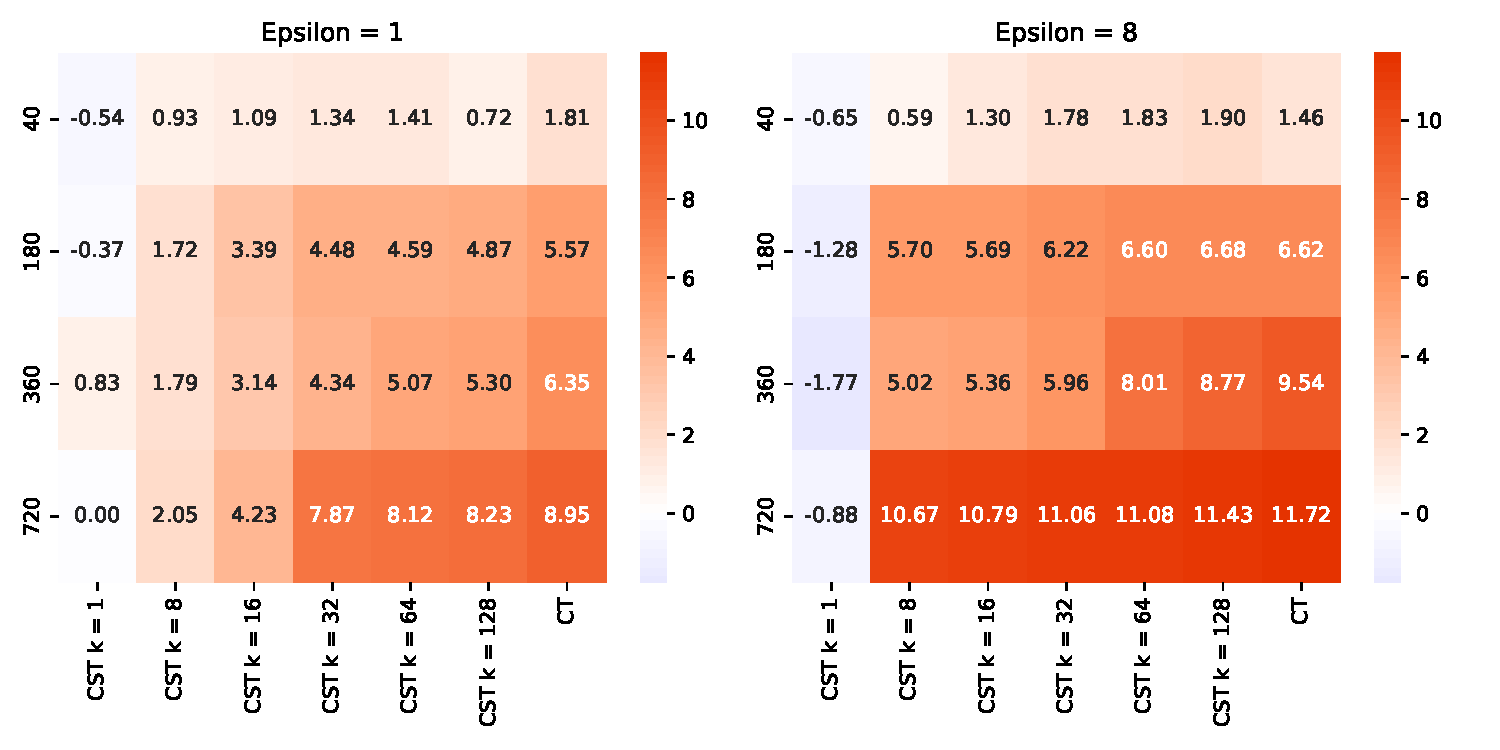
\includegraphics[width=7cm]{latex/fig/heatmap_semantic_sim_2.pdf}
    \caption{Semantic similarity improvement over SanText (\%). \clusant abbreviated by CST, CusText by CT. Horizontal axis varies parameter $k$ of \clusant. Vertical axis varies the number of clusters. Same axes apply for the other heatmaps as well. Unless otherwise mentioned, the higher, the better.}
    \label{fig:semsim_2}
\end{figure}


\begin{figure}[ht]
    \centering
    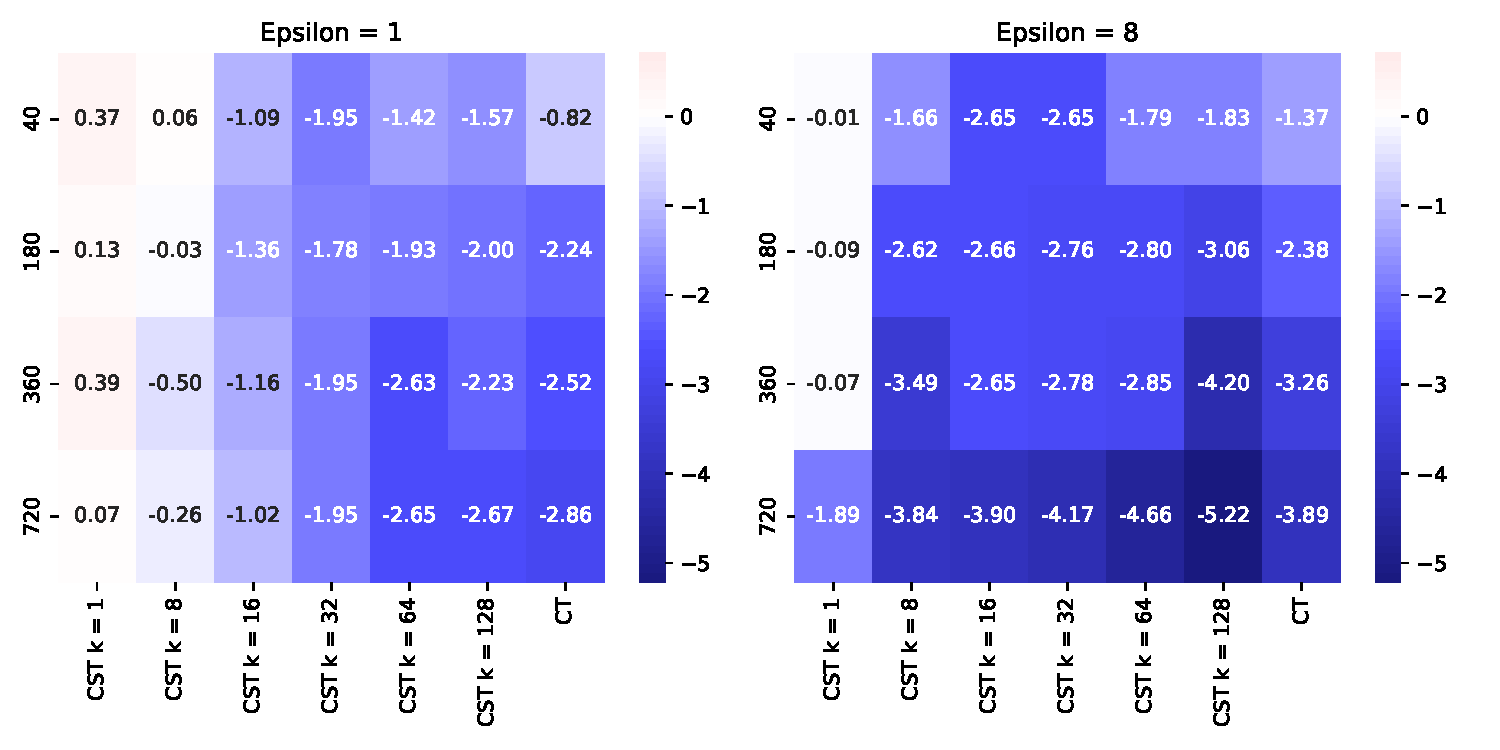
\includegraphics[width=7cm]{latex/fig/heatmap_perplexity_2.pdf}
    \caption{Peplexity improvement over SanText (\%); the lower, the better}
    \label{fig:perplexity_2}
\end{figure}


\begin{figure}[ht]
    \centering
    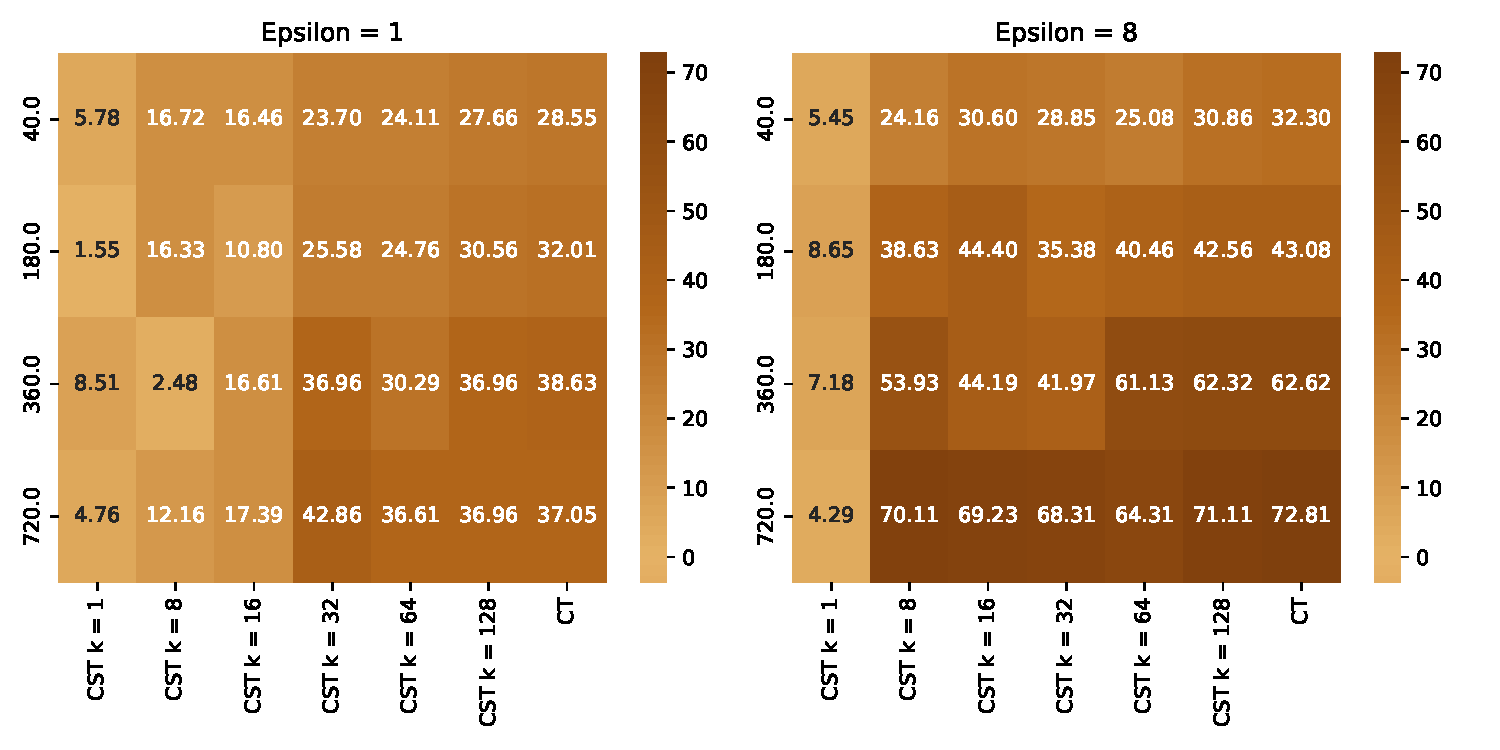
\includegraphics[width=7cm]{latex/fig/heatmap_common_sense_2.pdf}
    \caption{Common sense improv. over SanText (\%)}
    \label{fig:common_sense_2}
\end{figure}


\begin{figure}
    \centering
    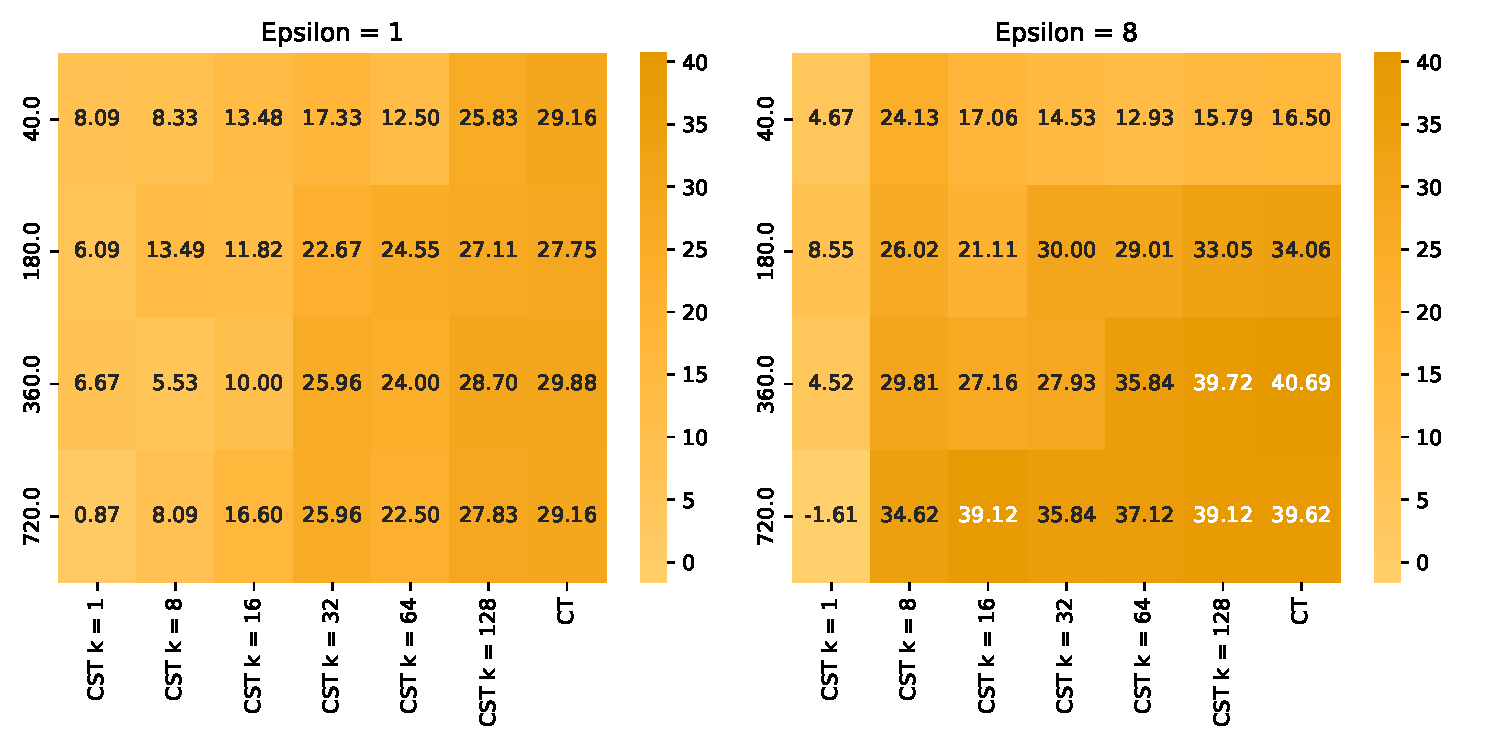
\includegraphics[width=7cm]{latex/fig/heatmap_coherence_2.pdf}
    \caption{Coherence improvement over SanText (\%)}
    \label{fig:coherence_2}
\end{figure}










\paragraph{Numerical Results}
We show partial experimental results, in Figures~\ref{fig:semsim_2}, \ref{fig:perplexity_2}, \ref{fig:common_sense_2}, \ref{fig:coherence_2} 
and full results in Figures~\ref{fig:semsim}, \ref{fig:perplexity}, \ref{fig:grammar}, \ref{fig:common_sense}, \ref{fig:coherence}, \ref{fig:cohesiveness} in the Appendix. 
The figures show improvements achieved by \clusant in terms of semantic similarity, perplexity, common sense, coherence, cohesiveness, and grammar over SanText. 
For all metrics except perplexity, higher scores are better, while for perplexity, lower scores are preferred.
We abbreviate \clusant by CST and CusText by CT. 
We consider CT as a special version of \clusant where $k=\infty$.

We plotted the number of clusters on the vertical axis and the centroid pushing factor $k$ of \clusant on the horizontal axis, creating heatmaps for each $\epsilon$ value considered: 0.5, 1, 2, 4, 8, 16. Due to space constraints, we only show results for $\epsilon=1$ and $\epsilon=8$ here and include the rest in the Appendix. 

For all $\epsilon$ values, as $k$ increases (moving right in the maps), the semantic similarity improvement (over SanText) increases. Additionally, as the number of clusters increases (moving down), semantic similarity improvement also increases.

The most significant improvement of \clusant over SanText is observed for $\epsilon = 8$ and 720 clusters. Generally, the more clusters used, the greater the improvement over SanText. For $\epsilon = 16$, the improvement in semantic similarity for \clusant over SanText is not as pronounced as for $\epsilon = 8$. This is because, while the semantic similarity of sanitized text to the original text for \clusant approaches 1 for this $\epsilon$ (the highest value possible, being a cosine similarity), the semantic similarity for SanText also increases for larger $\epsilon$ values, resulting in a slightly reduced improvement margin.

\looseness=-1
Similar trends are observed for perplexity, common sense, and coherence, as well as for grammar and cohesiveness (detailed in Appendix). As the number of clusters and $k$ increase, \clusant's performance improves significantly over SanText, approaching that of CusText. While CusText shows better performance across metrics, it is only marginally better than \clusant. However, this comes at the cost of weaker privacy guarantees.
% , as explained previously.
We note that these metrics represent general trends; as LLM judgments can be noisy, smaller $k$ values may occasionally yield better results.




\section{Conclusion}
We introduced \clusant, a novel framework for text sanitization that achieves metric local differential privacy (MLDP). % that addresses the need for effective privacy-preserving methods in text processing. 
\clusant comprises token clustering and token sanitization, leveraging Large Language Models to generate substitute tokens, which are then clustered, and sanitized using a MLDP algorithm.
Our MLDP framework encompasses, and gives a range of privacy-utility tradeoffs via tuneable parameters,  between state-of-the-art algorithms  SanText and CusText. % under specific parameters, balancing the privacy-utility tradeoff. 
This enables \clusant's users to achieve strong privacy or high utility as required. 
Our framework achieves MLDP guarantees regardless of the clustering, allowing for plug-and-play (and future optimization) of %privacy guarantees are independent of the clustering method, allowing 
this component in our framework. 
%Future work can optimize these algorithms to enhance \clusant's performance further. 
In summary, \clusant advances the area of privacy-preserving text processing, 
offering a robust, tuneable solution for handling sensitive text. % across diverse contexts.

% Our framework's privacy guarantees are independent of the clustering method, allowing for various clustering algorithms. Future work can optimize these algorithms to enhance \clusant's performance further. Overall, \clusant advances privacy-preserving text processing, offering a robust solution for handling sensitive data across diverse contexts.


% \section{Conclusions}
% We introduced \clusant, a novel framework for text sanitization that addresses the need for effective privacy-preserving methods in text processing. 
% Our framework consists of two key components: token clustering and token sanitization. 
% By leveraging Large Language Models (LLMs) to create a set of potential substitute tokens, we then meaningfully cluster these tokens and utilize a metric LDP algorithm to sanitize sensitive tokens within the text.

% Our (M)LDP algorithm's flexibility allows it to emulate existing state-of-the-art (SOTA) algorithms like SanText and CusText under specific parameter settings. This adaptability facilitates the privacy-utility tradeoff, enabling \clusant to achieve either strong privacy similar to SanText or high utility akin to CusText, depending on the chosen parameters.

% To rigorously benchmark \clusant, we used evaluation metrics that focus on semantic similarity and language naturalness. 
% Our experimental results demonstrate that \clusant offers a sensible balance between privacy and utility.

% We emphasize that the privacy guarantees of our token sanitization algorithm are regardless of the clustering algorithm, allowing for flexible plug-and-play of different clustering methods. Future work may explore optimizing clustering algorithms to further enhance \clusant's performance in various application domains. Overall, we believe \clusant represents a significant advancement in the field of privacy-preserving text processing, offering a promising solution for handling sensitive data across diverse textual contexts.





% \newpage


\newpage
\section*{Limitations}

\begin{itemize}
\setlength\itemsep{0em}
    \item We inherit some limitations of SanText/CusText. In particular, sanitizing a text by sanitizing individual tokens can lead to mistakes. For example, when a token has two different meanings in different contexts, the token sanitization may not know which meaning it should take. 
    While we use a sentence embedder that generates different embeddings for `London, Ontario' and `London, England,' it is not helpful for distinguishing `Jordan' as a country from the name `Jordan.' 
    To achieve this, the embedder would need to consider the meaning of the entire passage. 
    However, accomplishing this is challenging and requires further work. We believe our framework can be improved in follow-up studies by considering token context in our clustering and text sanitization.
    
    % While we attempt to remedy this by creating a sensible prompt when generating the augmented set $X'$ of sensitive tokens (in the Appendix), the full details of how to accomplish this remain far from obvious. 

    \item While we improved the sensitive token set and multi-word embedding in our framework, we tested only one clustering method (that of CusText's) and primarily used Euclidean distances. A future direction is to enrich our framework by exploring and comparing other clustering methods and distance metrics. 

    % (in line with SanText/CusText). 
    %While \clusant's privacy guarantees works for any clustering method, we believe that having a good clustering is essential for good utility. We plan to experiment with other clustering methods in future work.
    % \item We utilized direct metrics to measure the utility of the sanitized text. %, as opposed to previous work that measured performance in specific downstream tasks. 
    % This approach allowed for a more straightforward and transparent comparison of \clusant with previous methods. In follow-up works, we plan apply our approach to specific downstream tasks.
\end{itemize}

% From: \url{https://aclrollingreview.org/cfp#long-papers}

% Limitations (required section)
% Authors are required to discuss the limitations of their work in a dedicated section titled “Limitations”. This section should be included at the end of the paper, before the references, and it will not count toward the page limit. This includes both, long and short papers. Papers without a limitations section will be desk rejected. Note, prior to the December 2023 cycle, this was optional.








\bibliography{privacylm}


% Bibliography entries for the entire Anthology, followed by custom entries
%\bibliography{anthology,custom}
% Custom bibliography entries only
% \bibliography{custom}

\appendix

\section{Differential Privacy Definition}


\begin{definition}(\(\epsilon\)-Differential Privacy \cite{dwork2006differential})
Given a privacy parameter \(\epsilon \geq 0\), for any two adjacent inputs \(x, x' \in X\) and each potential output \(y \in Y\), a randomized mechanism \(M\) satisfies \(\epsilon\)-differential privacy (DP) if it ensures that
\[
\frac{\Pr[M(x) = y]}{\Pr[M(x') = y]} \leq e^{\epsilon}.
\]
\end{definition}


\section{SanText and CusText}

\subsection{SanText}


Below, we detail the operational steps of the token sanitization mechanism \( M \) of SanText when processing an input token \( x \):

\begin{enumerate}
    \item \( M \) is parameterized by the privacy parameter \( \epsilon \) and employs a metric $d$ to measure distances between tokens.
    \item The utility function \( u \) is defined such that \( u(x, x) = -d(x, x) \). Under this definition, \( M \) selects an output from \( Y \) based on the exponential mechanism (Def.~\ref{def:expmech}) tailored for the specified \( \epsilon \), but with the utility sensitivity \( \Delta u \) replaced by \( 1 \).
\end{enumerate}

\subsection{CusText}

We describe CusText's token sanitization algorithm $M:X'\rightarrow X$ for input token $x$. 

\begin{enumerate}
    \item $M$ is parametrized by the formed clusters, a distance $d$, and the privacy parameter $\epsilon$.
    \item Let $C\subseteq X$ be the cluster $x$ belongs in.
    \item Let utility $u:C \times C \rightarrow \mathbb{R}$ be the negative of the normalised distance $u(x,y) = - \frac{d(x,y) - d_{\min}}{d_{\max} - d_{\min}}$ ($d_{\min} = \min_{x,y\in C}d(x,y)$ and $d_{\max}= \max_{x,y\in C}d(x,y)$), so that sensitivity $\Delta u = 1$. 
    \item Using the above utility function, replace $x$ with some token in $C$ via the exponential mechanism (Def.~\ref{def:expmech}) for privacy $\epsilon$.
\end{enumerate}

We present the proof that CusText cannot achieve standard (M)LDP when there is more than one cluster.
\begin{proof}
    We prove first for LDP.  Suppose for contradiction that there exists $\epsilon\in \mathbb{R}$ such that $M$ satisfies $\epsilon$-LDP. Then for all $x, x' \in X', y \in X$, this inequality must hold: 
    $$
        \Pr(M(x) = y) \leq e^\epsilon \Pr(M(x') = y)
    $$
    Since there are at least two clusters, there must exist $x, x' \in X'$ that belong in different clusters. Let $y$ be a token in the cluster of $x$, which means $y$ is not in the cluster of $x'$. This means that $\Pr(M(x) = y) > 0$ and $e^\epsilon \Pr(M(x') = y) = e^\epsilon \cdot 0 = 0$. Thus the above inequality cannot hold, which is a contradiction, and thus there is no  $\epsilon$ for which $M$ is $\epsilon$-LDP.

     The proof for metric LDP follows since if $M$ is $\epsilon$-metric LDP then  $M$ is $\epsilon\cdot \Delta u$-LDP. Since the lexicon is finite, $\Delta u$ maximises over a finite set and is also finite. Thus, if $M$ is $\epsilon$-metric LDP then it is $\epsilon'$-LDP for some finite $\epsilon'$ (which we just proved is impossible).    
\end{proof}


\section{Detailed Experimental Results}

Here we give the detailed prompt for obtaining the extended set $X'$ of sensitive tokens using GPT-4o.

{\em
\begin{quote}
If I give you a word or phrase, example ``southern norrland,'' can you give me 100 similar words/phrases of the same category?

For example:
\begin{itemize}
    \item If it is a location, give me other locations that are similar in nature.
    \item If it is an organization, give me other organizations that are similar.
    \item If it is an object, give me other objects that are similar.
\end{itemize}

The similarity should be in terms of the category and characteristics of the entity. The words you give should make sense if used as a replacement for the original word/phrase in a similar context.

Format output as a list of words/phrases:
\[
[\text{word/phrase1, word/phrase2, ...}]
\]

Here the context that "\{search\_phrase\}" was used in: "\{context\}".
\end{quote}
}


For example, when the search phrase was `sarpsborg city court (tingrett)' with its context in the TAB text, the output we received from GPT-4o was:

[`oslo district court', `bergen district court', `trondheim district court', `stavanger district court', `kristiansand district court', `tromsø district court', `drammen district court', `fredrikstad district court', `skien district court', `ålesund district court', `bodø district court', `hamar district court', `molde district court', `haugesund district court', etc].


Now we give detailed experimental results on 
semantic similarity (Figure~\ref{fig:semsim}),
perplexity (Figure~\ref{fig:perplexity}),
grammar (Figure~\ref{fig:grammar}),
common sense (Figure~\ref{fig:common_sense}), 
coherence (Figure~\ref{fig:coherence}), and 
cohesiveness (Figure~\ref{fig:cohesiveness}).
For perplexity we used GPT-2. To judge the grammar, common sense, coherence, and cohesiveness of santized text, we used GPT-4o, with the following prompt. 


{\em
\begin{quote}
Could you please evaluate the following passage for its grammar, common sense, coherence, and cohesiveness? Score it on a scale from 1 to 5, where 1 is the lowest (poor quality) and 5 is the highest (excellent quality).

You should score based on these criteria:
\begin{itemize}
    \item \textbf{Grammar}: Are the sentences structured correctly?
    \item \textbf{Common sense}: Does the content make logical sense in the real world?
    \item \textbf{Coherence}: Do the ideas flow logically from one sentence to another?
    \item \textbf{Cohesiveness}: Do all parts of the text come together in a unified whole?
\end{itemize}

Please ONLY respond in JSON format with the four keys 'grammar', 'common sense', 'coherence', and 'cohesiveness', each with a score attached to them.
\end{quote}
}


CluSanT's improvement over SanText generally increases with the number of clusters used. Increasing the number of clusters and parameter \(k\) significantly enhances CluSanT’s performance, approaching that of CusText. Although CusText performs better across metrics, it offers weaker privacy guarantees. Note that these metrics represent general trends, and due to noisy judgments from LLMs, smaller \(k\) values can sometimes yield better results.



\begin{figure*}
    \centering
    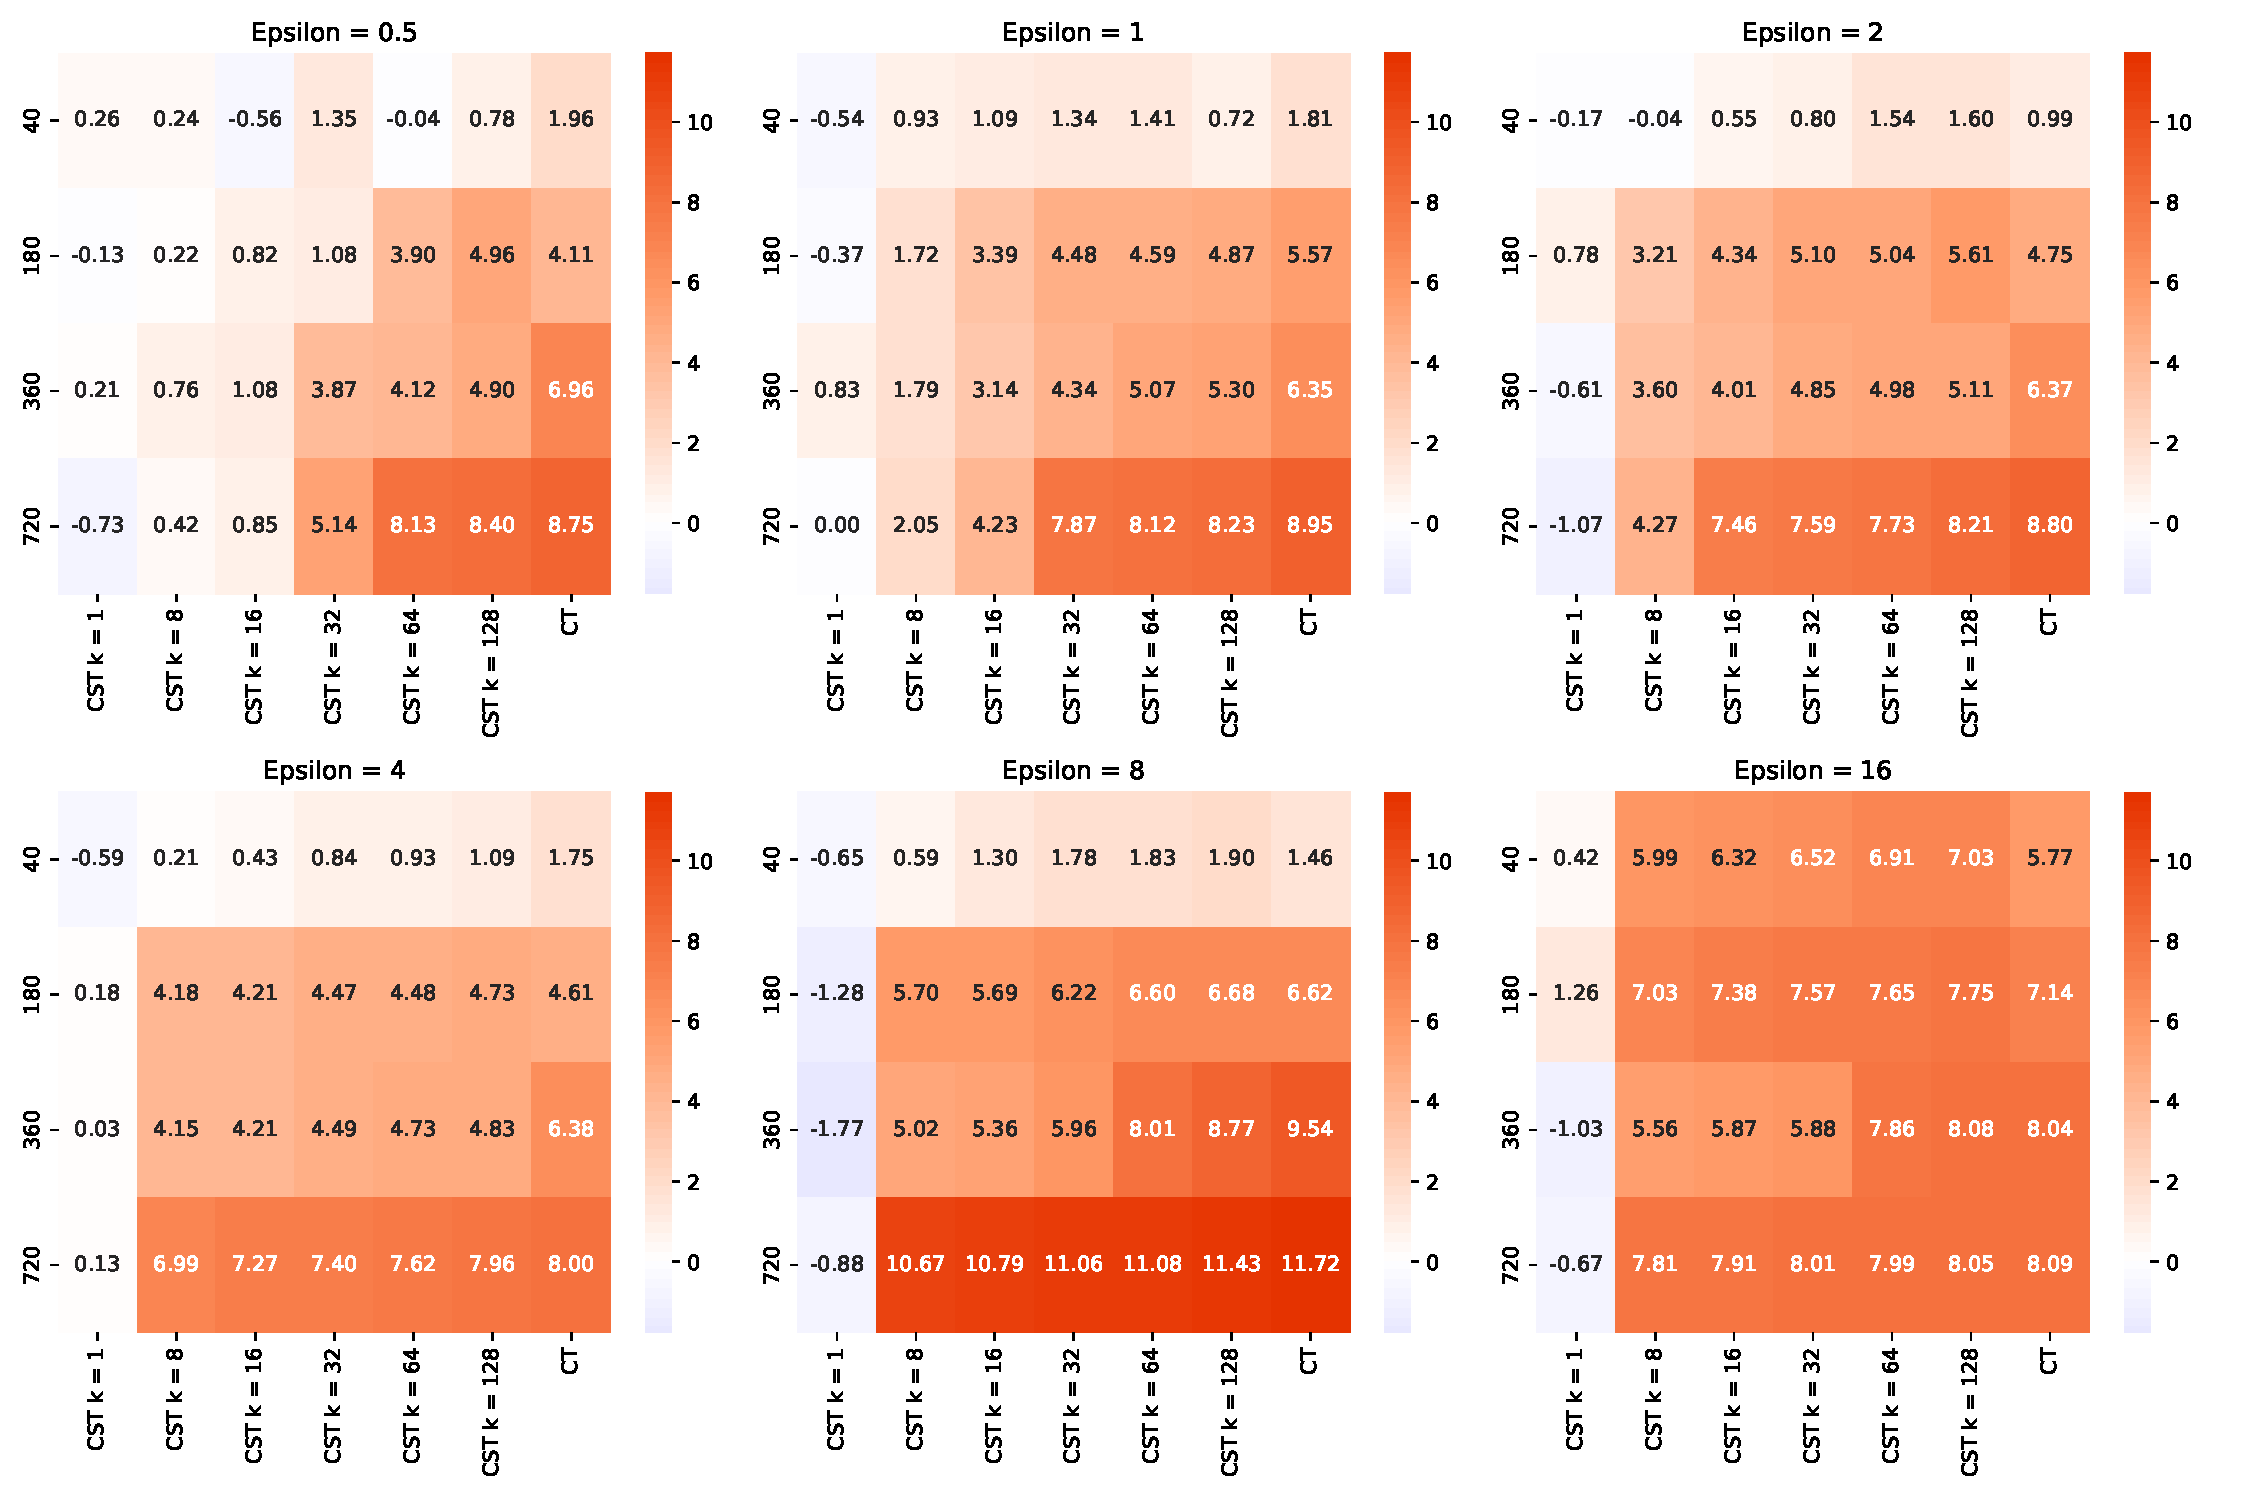
\includegraphics[width=15cm]{fig/heatmap_semantic_sim.pdf}
    \caption{Semantic similarity improvement over SanText (\%); the higher, the better. \clusant abbr. by CST and CusText by CT. Horizontal axis varies parameter $k$ of \clusant. Vertical axis varies the number of clusters. Same axes apply for the other heatmaps as well.}
    \label{fig:semsim}
\end{figure*}


\begin{figure*}
    \centering
    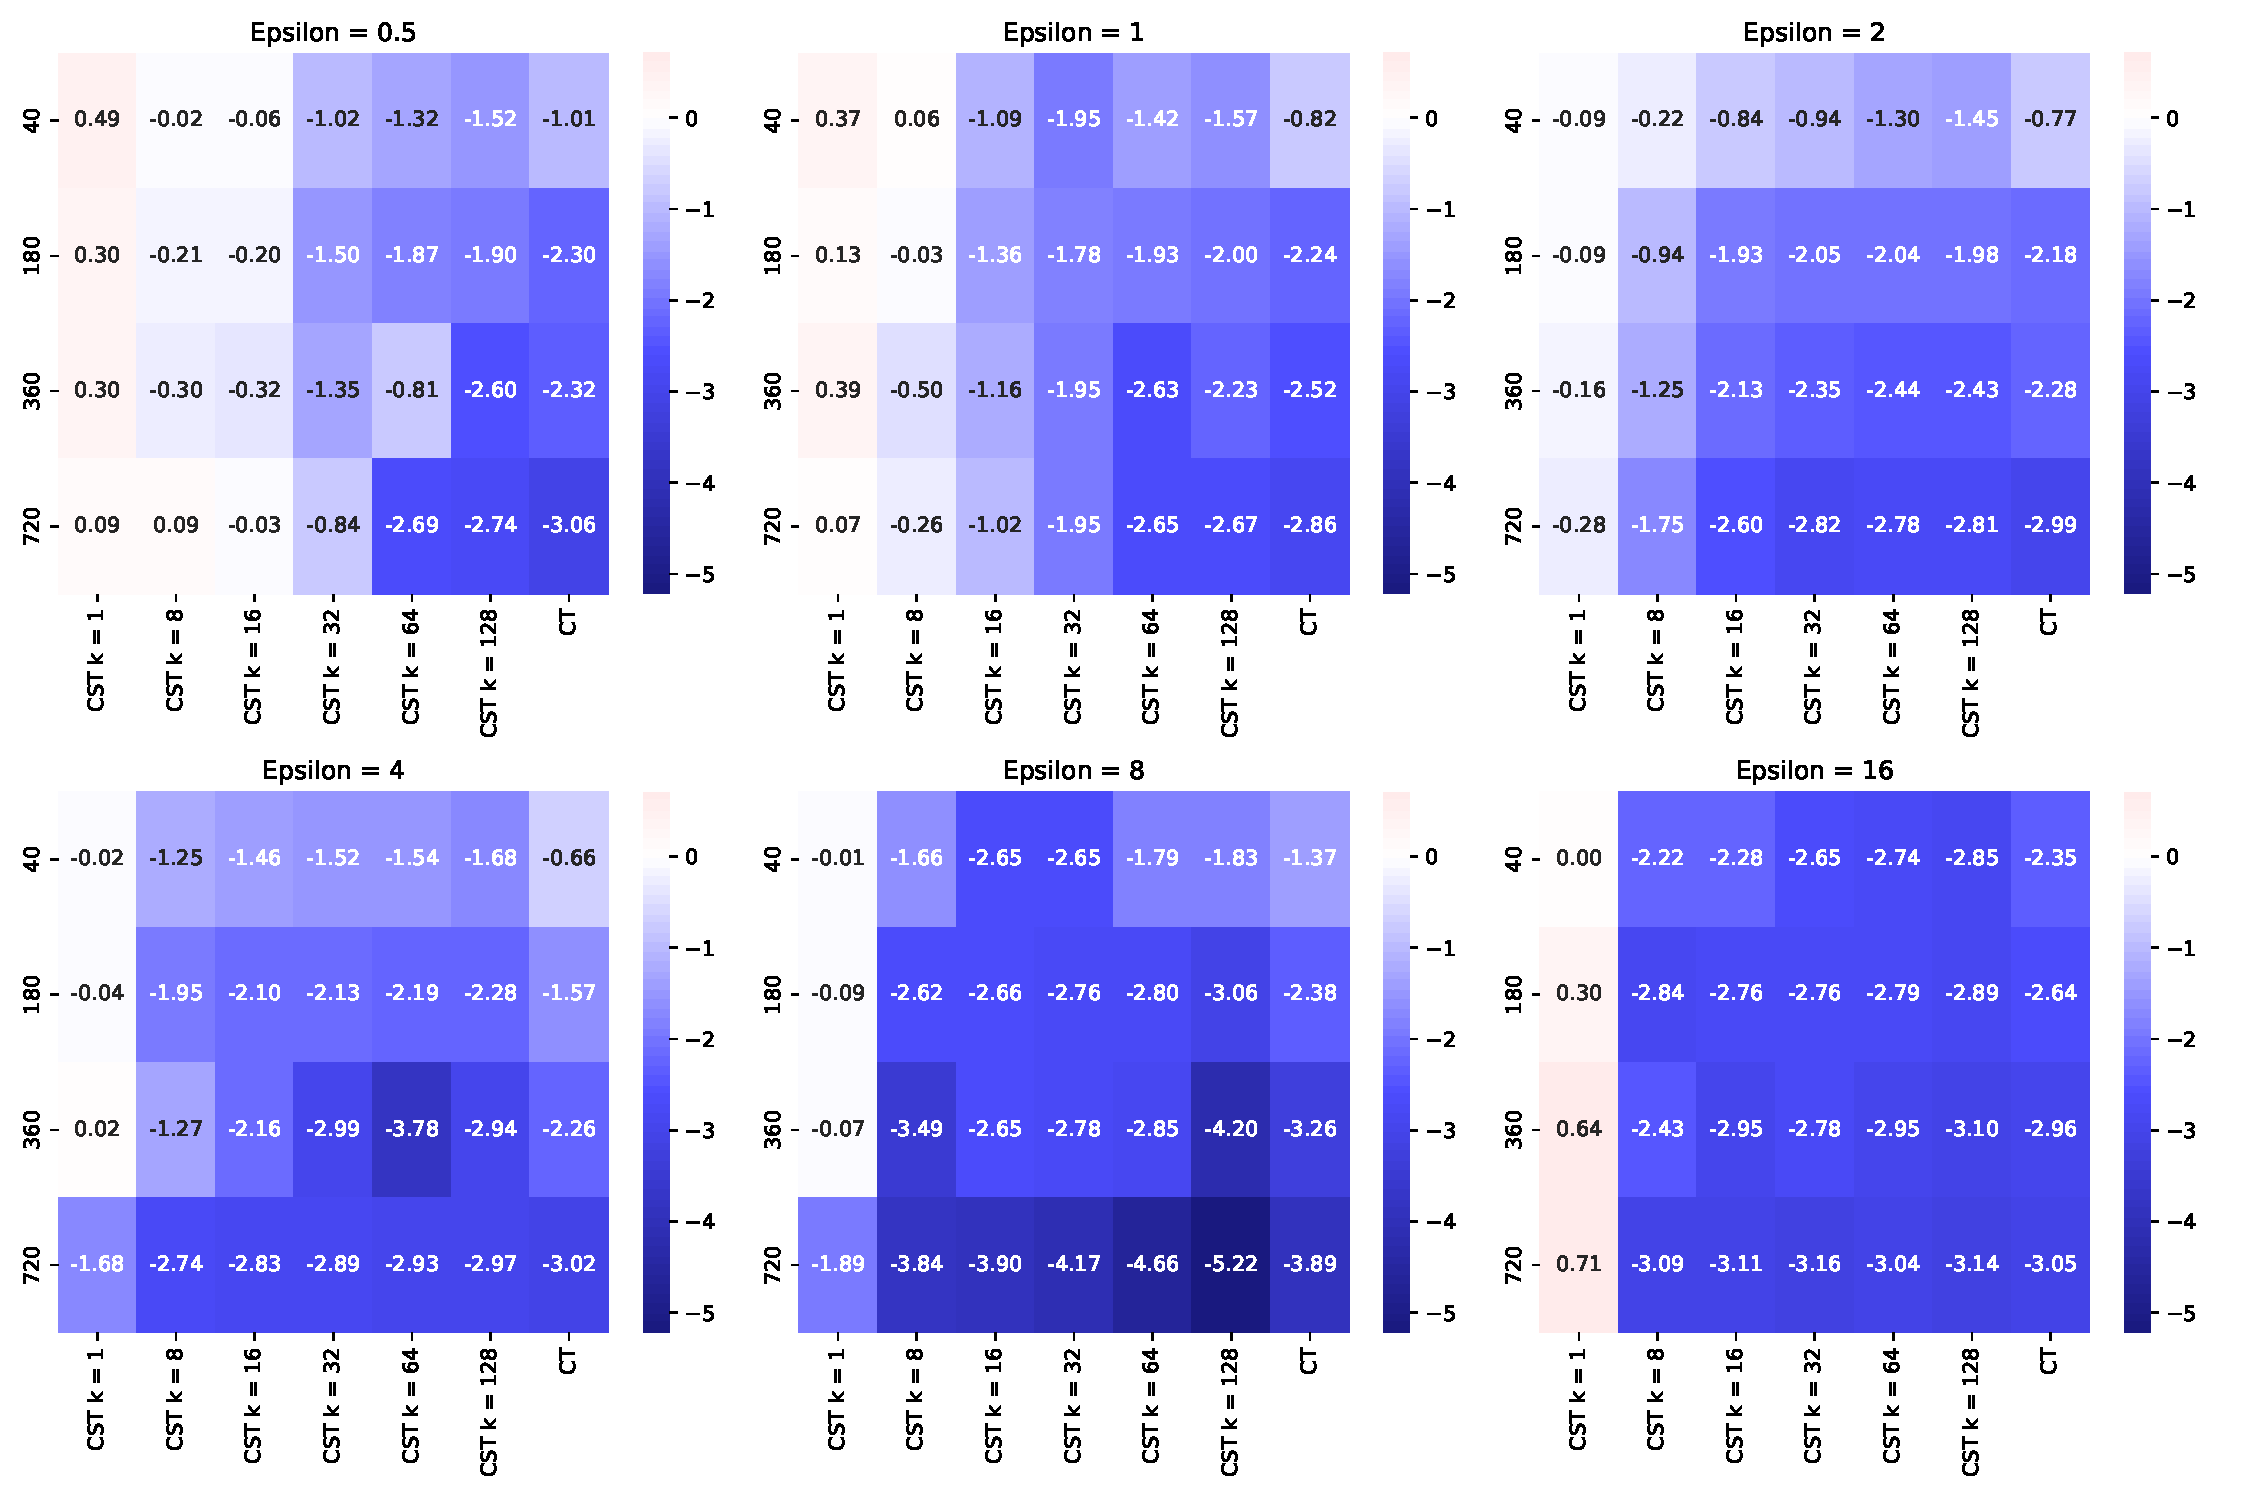
\includegraphics[width=15cm]{fig/heatmap_perplexity.pdf}
    \caption{Peplexity improvement over SanText (\%); the lower, the better.}
    \label{fig:perplexity}
\end{figure*}



\begin{figure*}
    \centering
    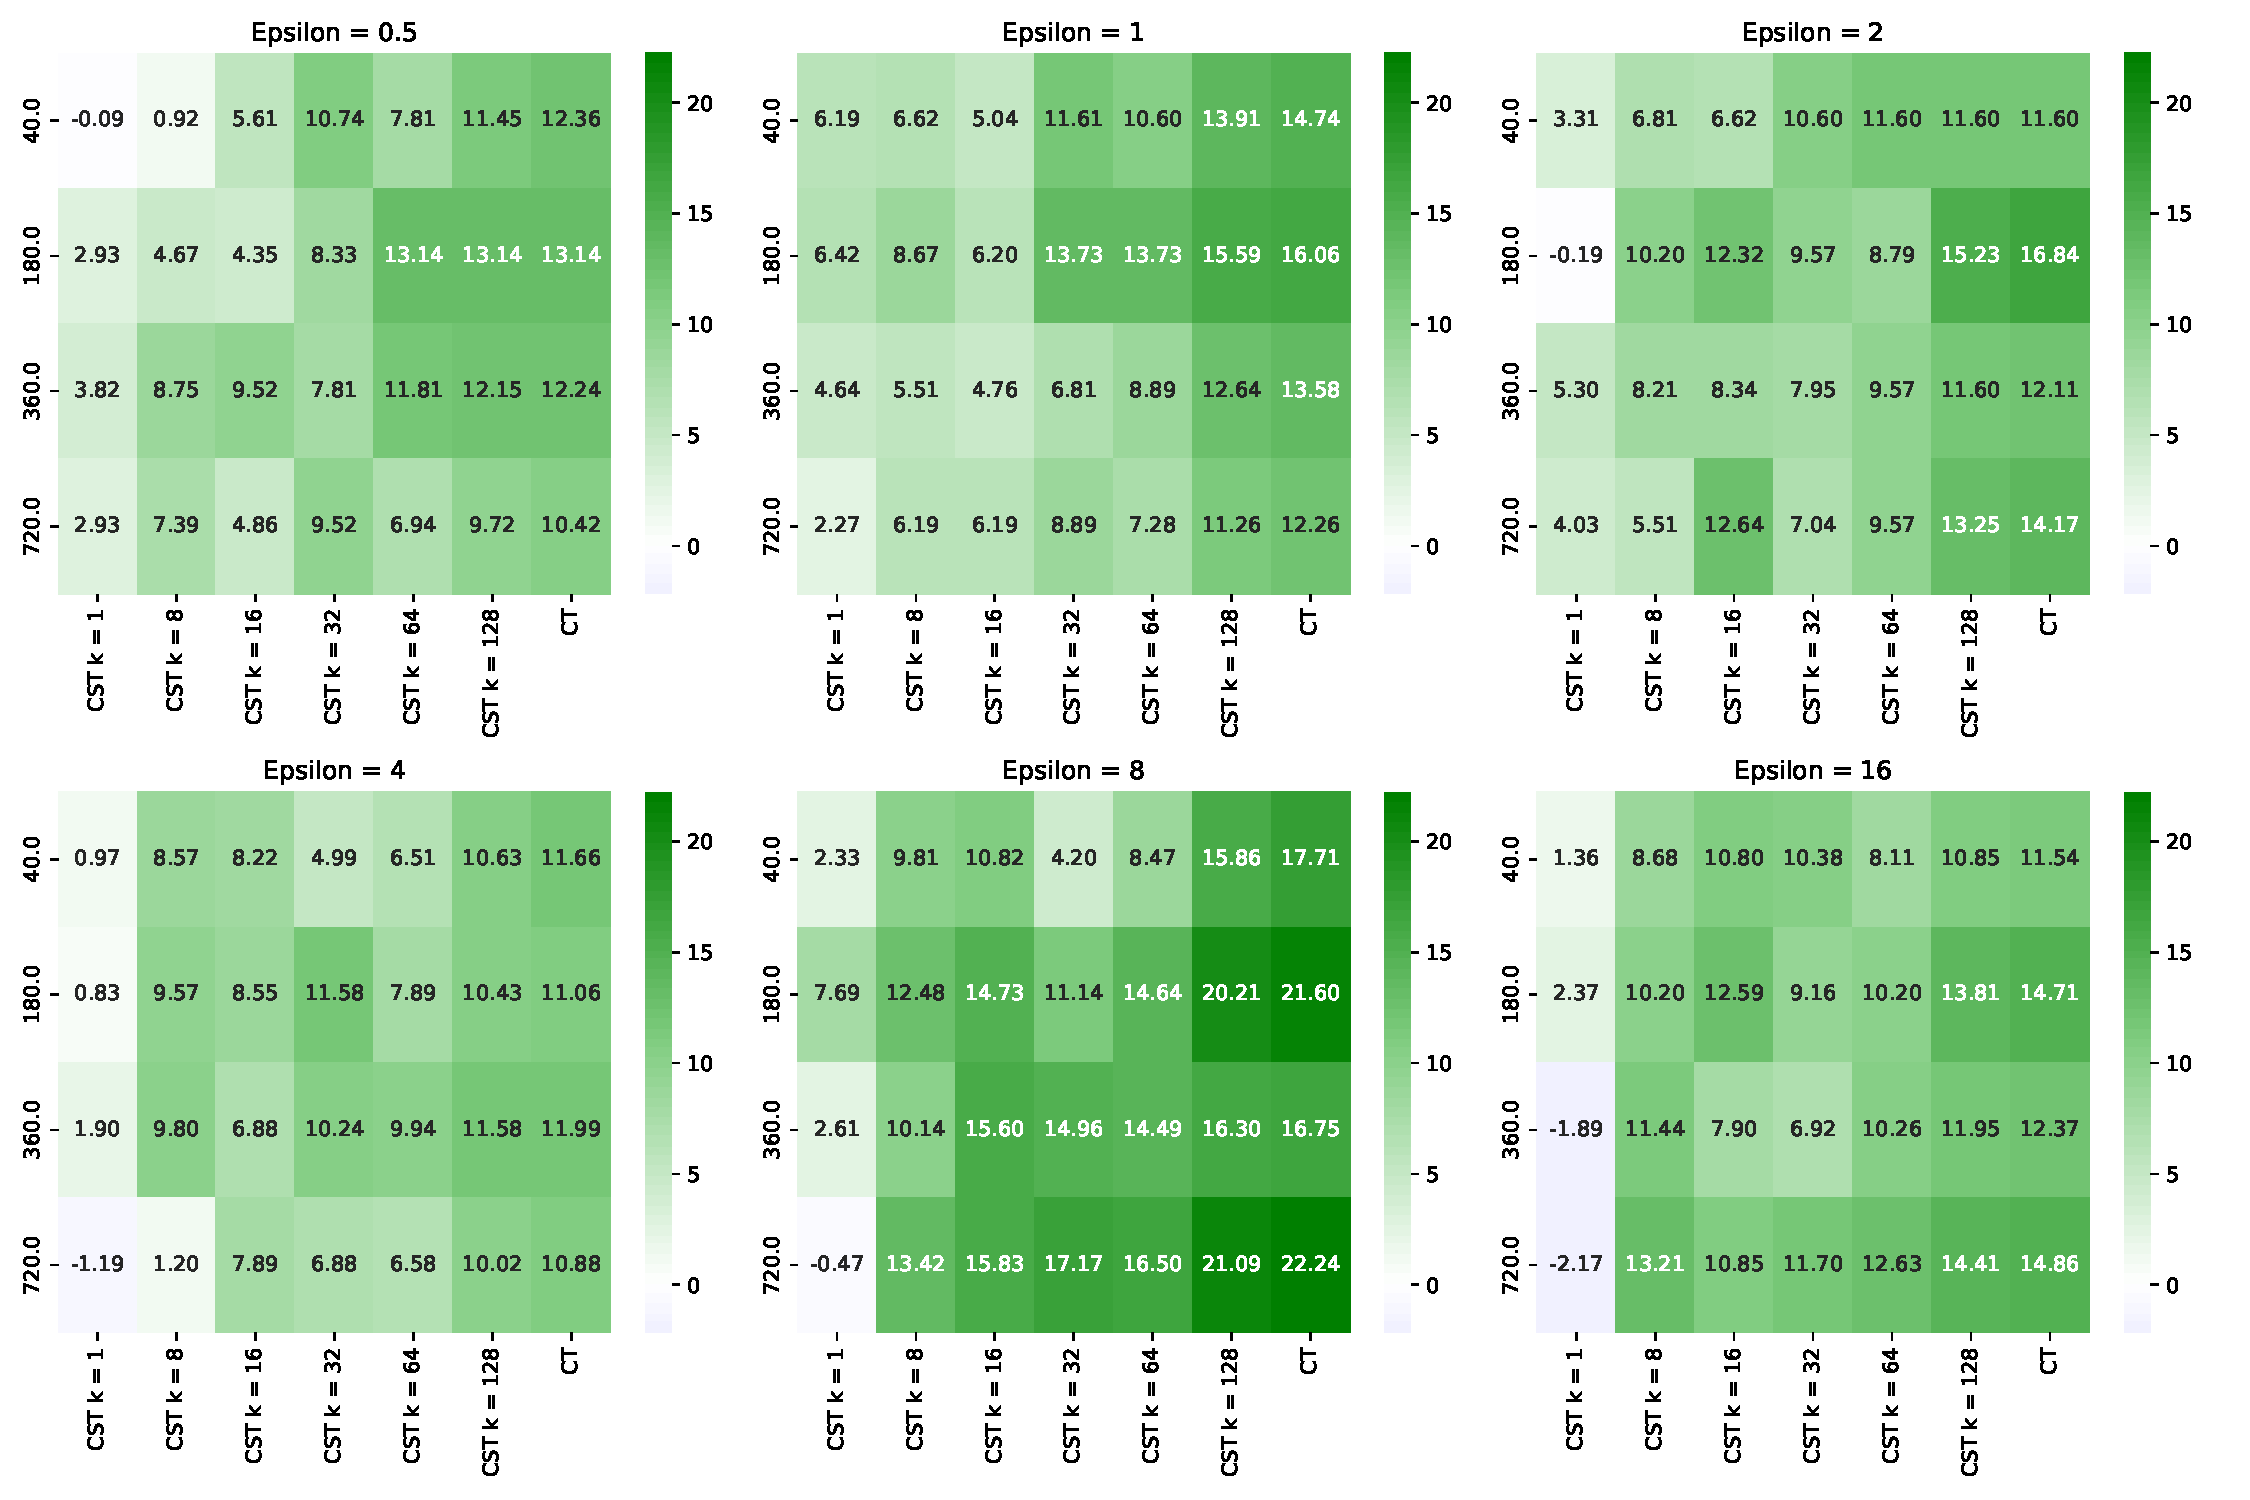
\includegraphics[width=15cm]{latex/fig/heatmap_grammar.pdf}
    \caption{Grammar improvement over SanText (\%); the higher, the better.}
    \label{fig:grammar}
\end{figure*}


\begin{figure*}
    \centering
    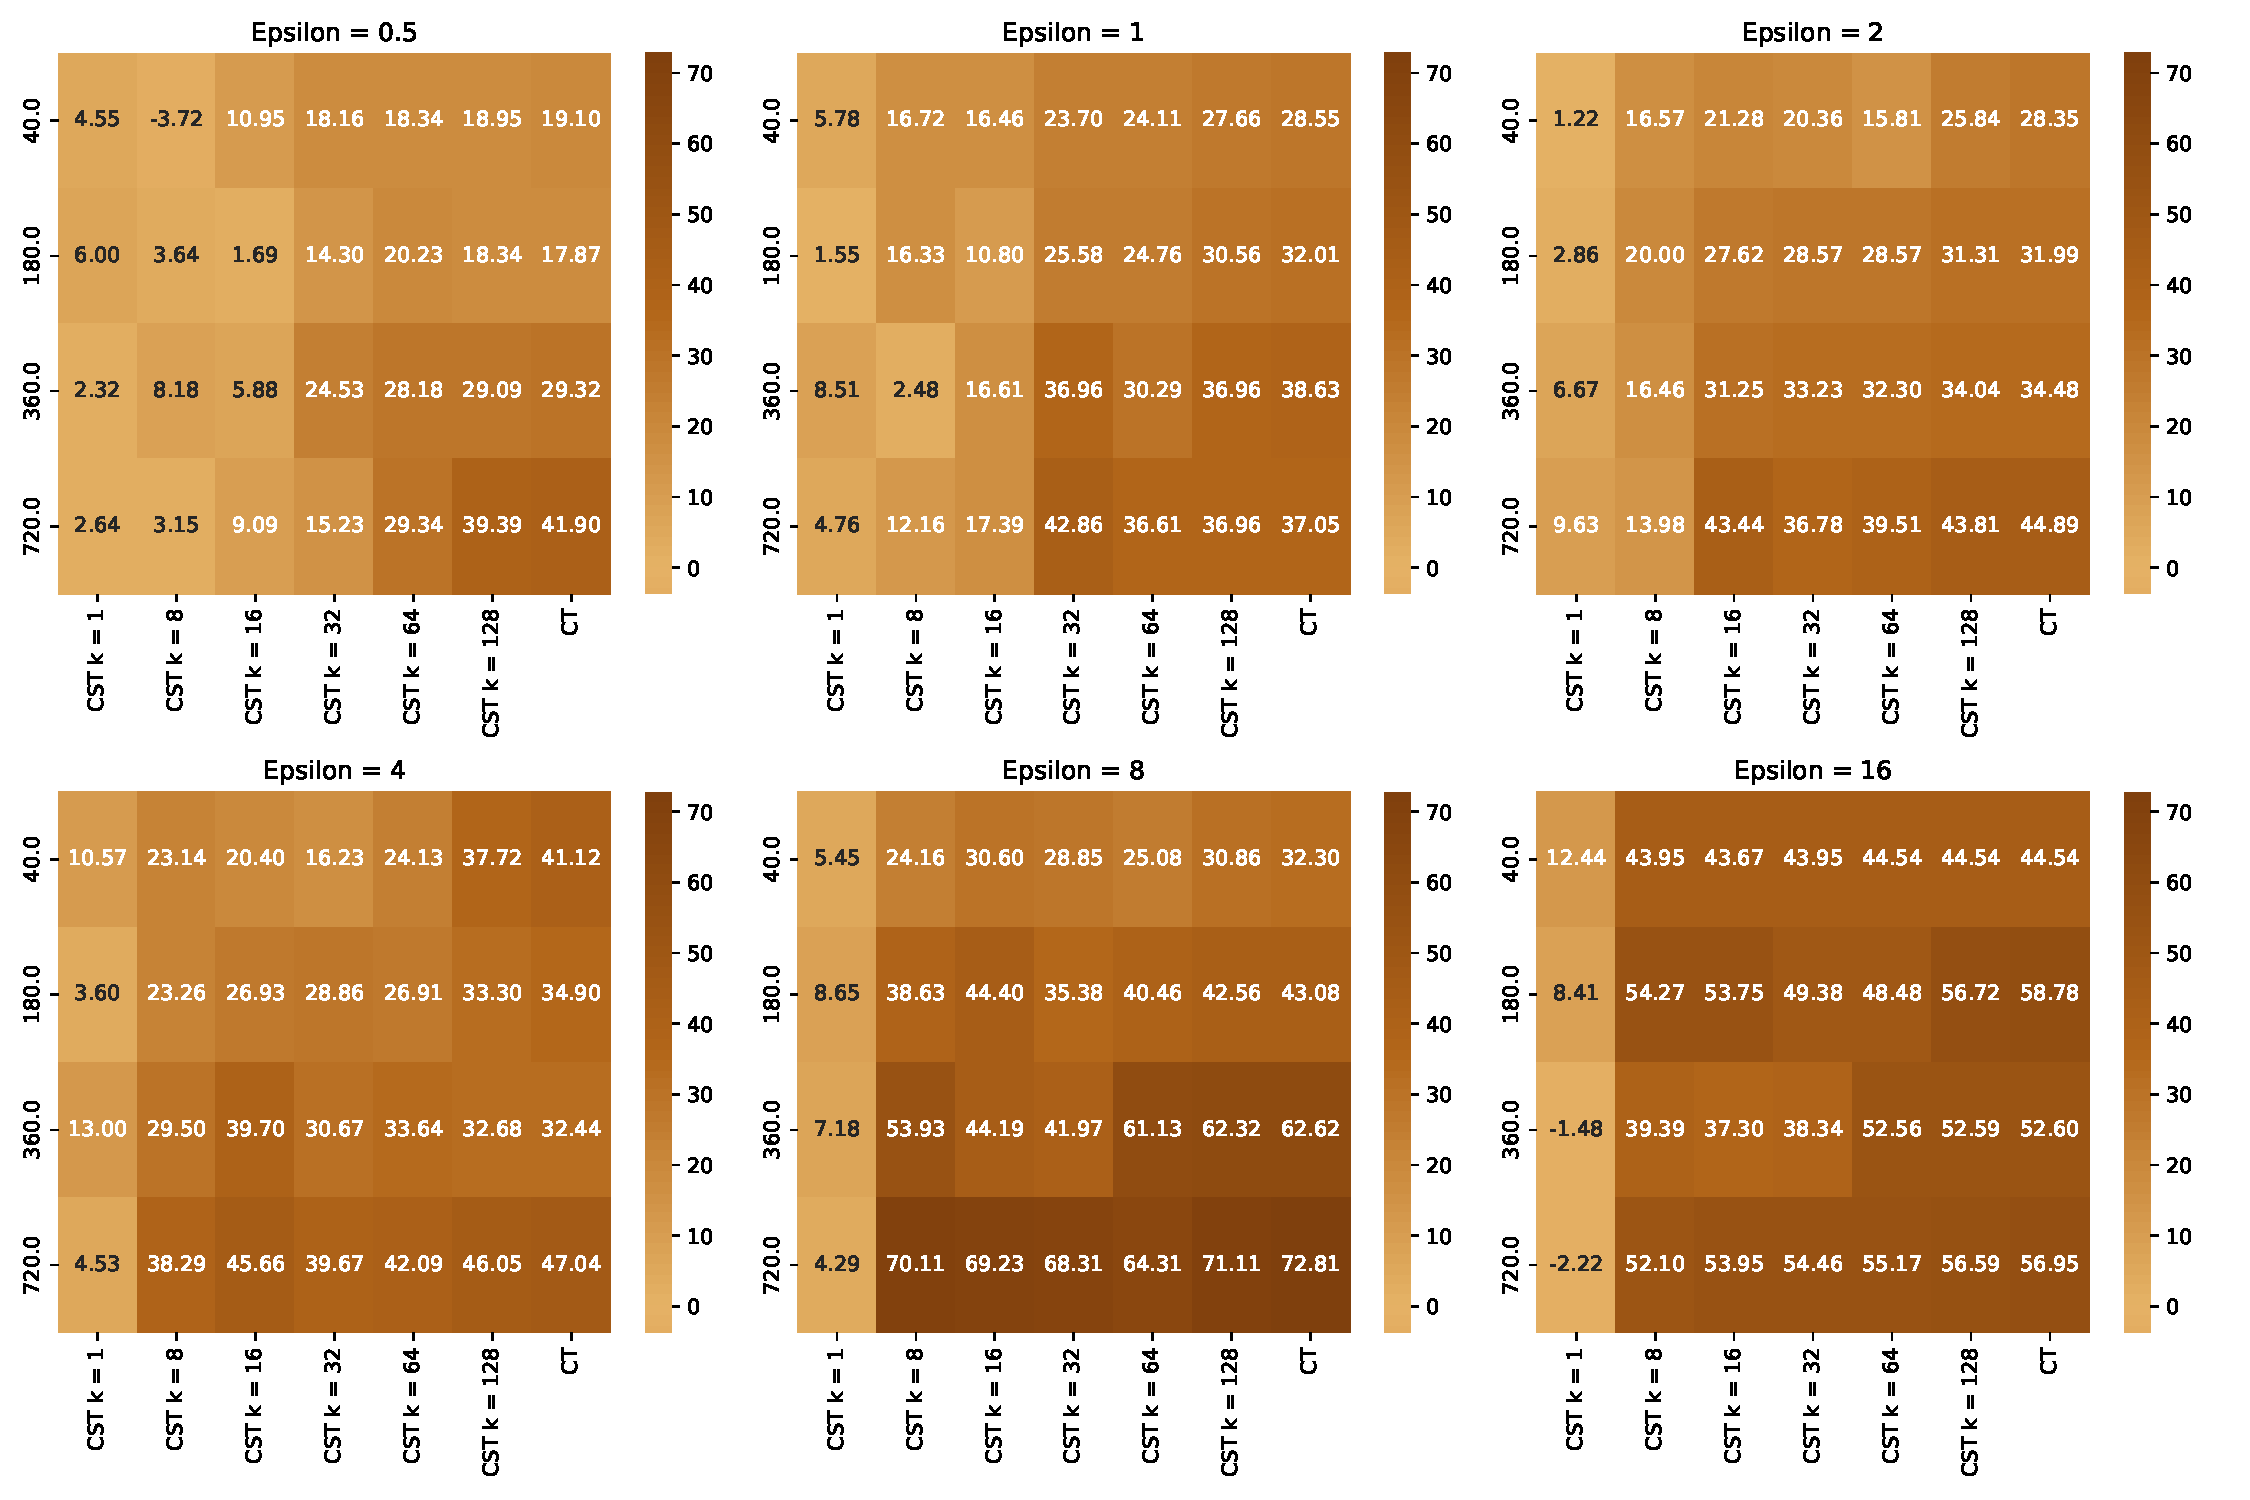
\includegraphics[width=15cm]{latex/fig/heatmap_common_sense.pdf}
    \caption{Common Sense improvement over SanText (\%); the higher, the better.}
    \label{fig:common_sense}
\end{figure*}


\begin{figure*}
    \centering
    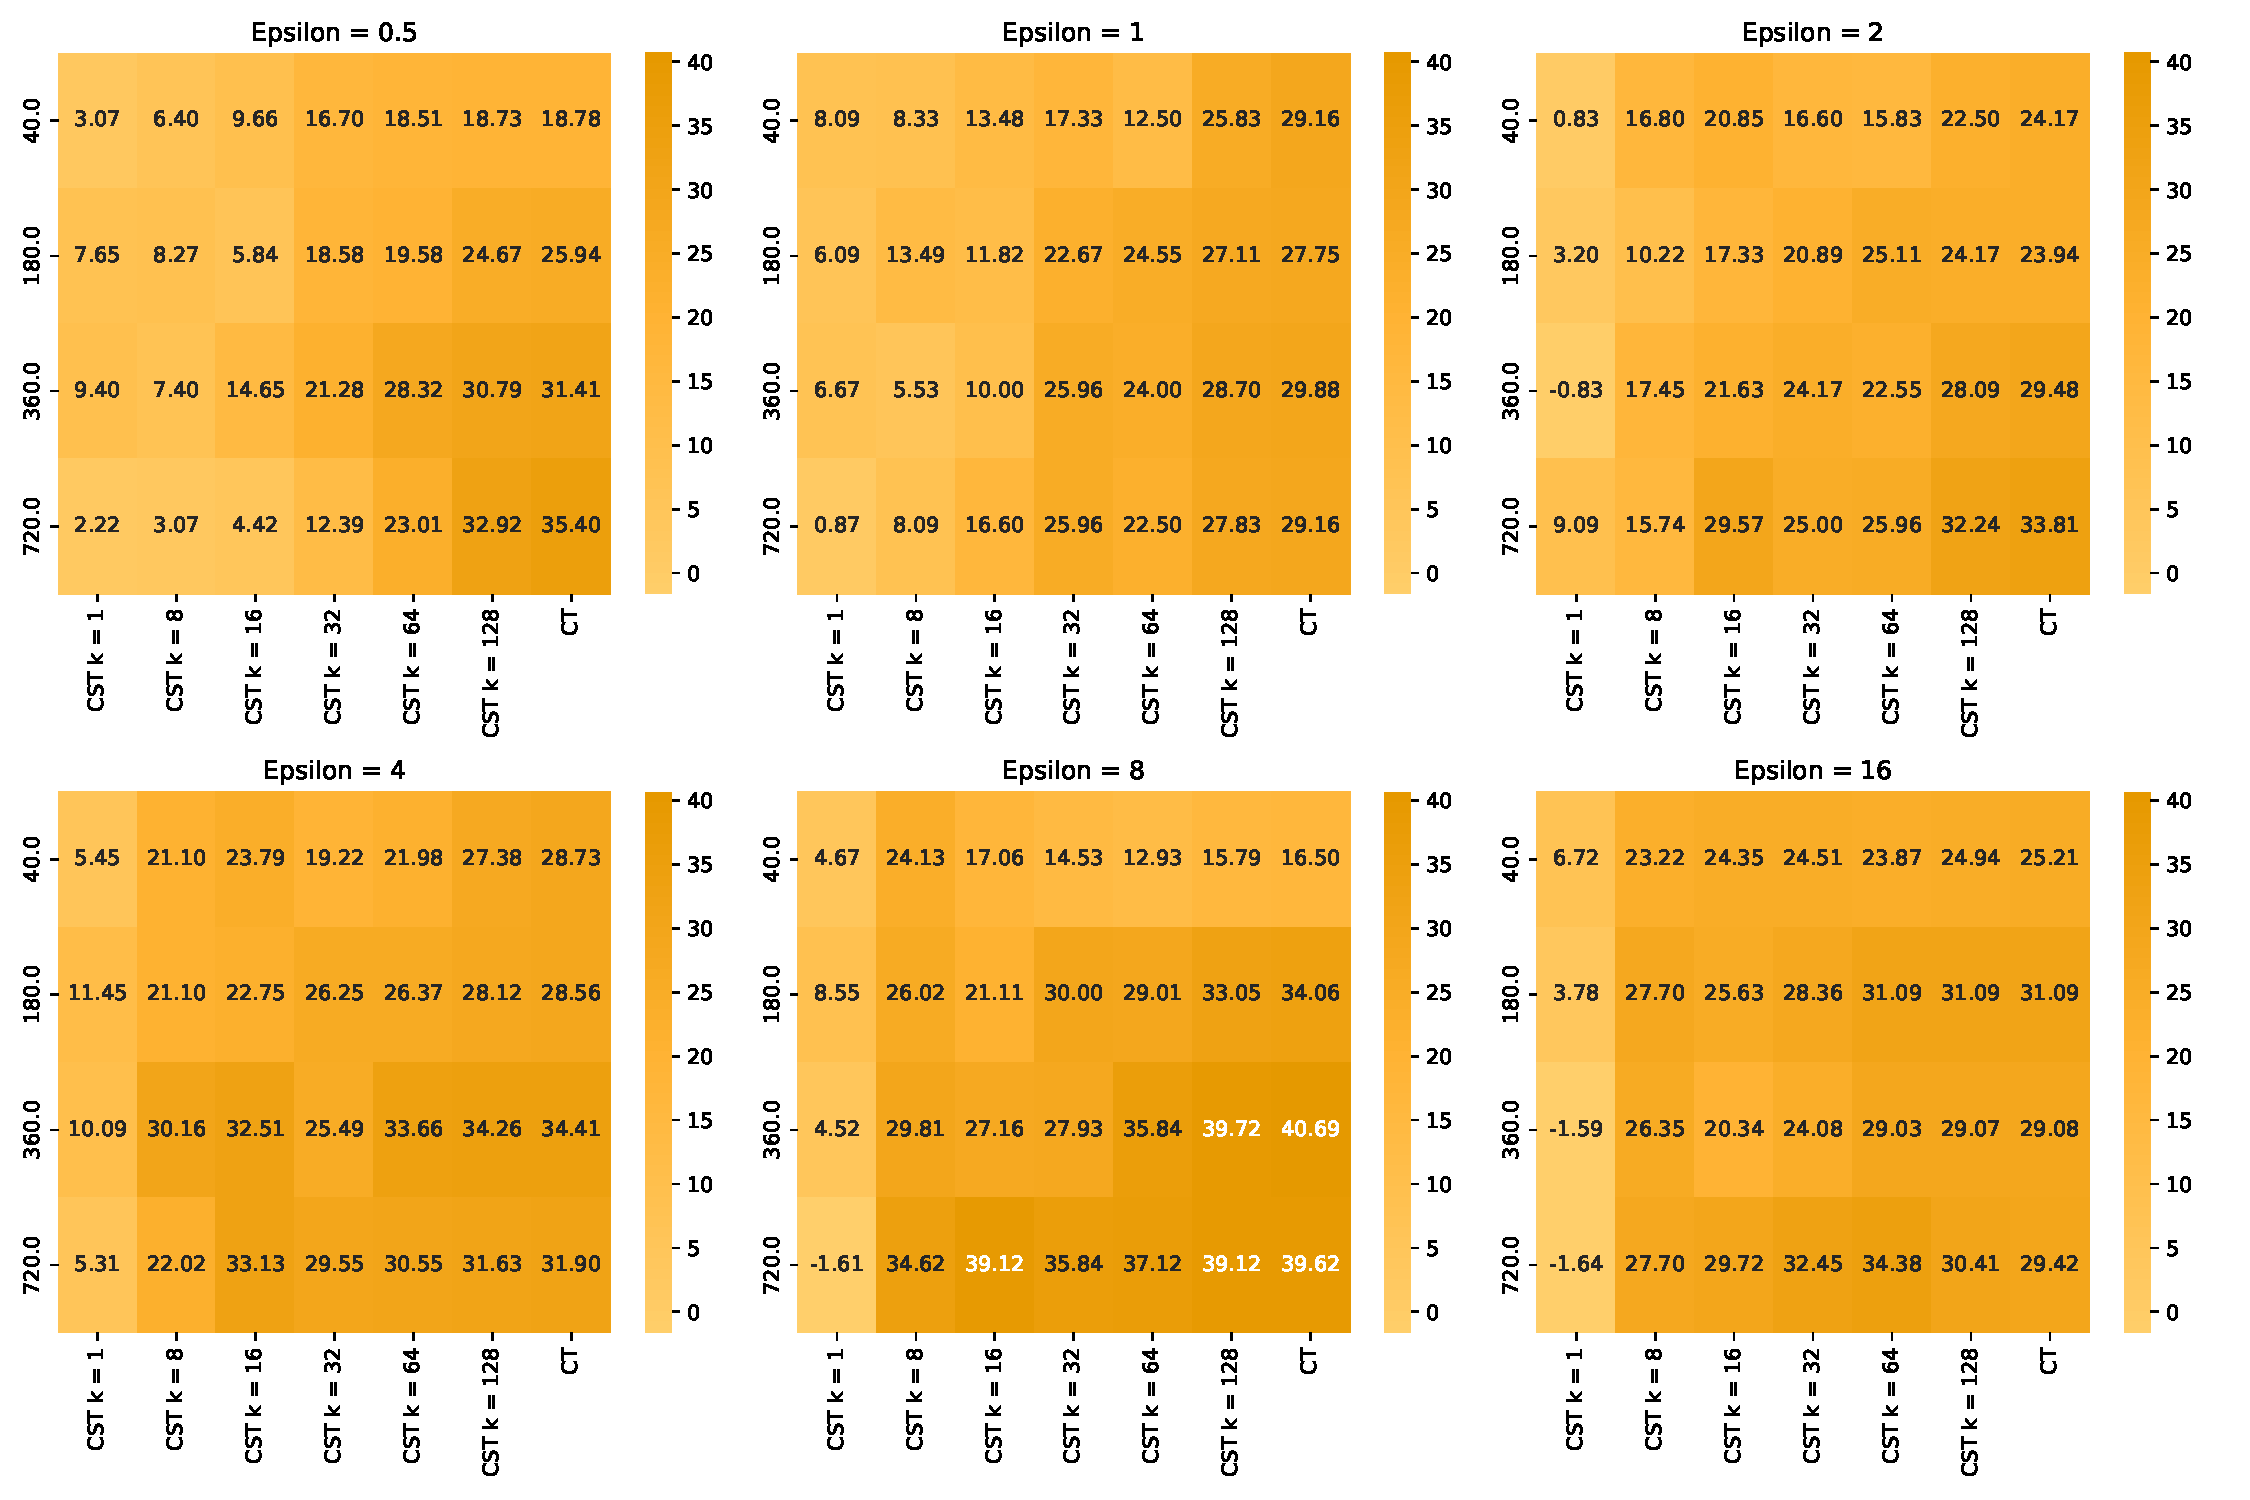
\includegraphics[width=15cm]{latex/fig/heatmap_coherence.pdf}
    \caption{Coherence improvement over SanText (\%); the higher, the better.}
    \label{fig:coherence}
\end{figure*}


\begin{figure*}
    \centering
    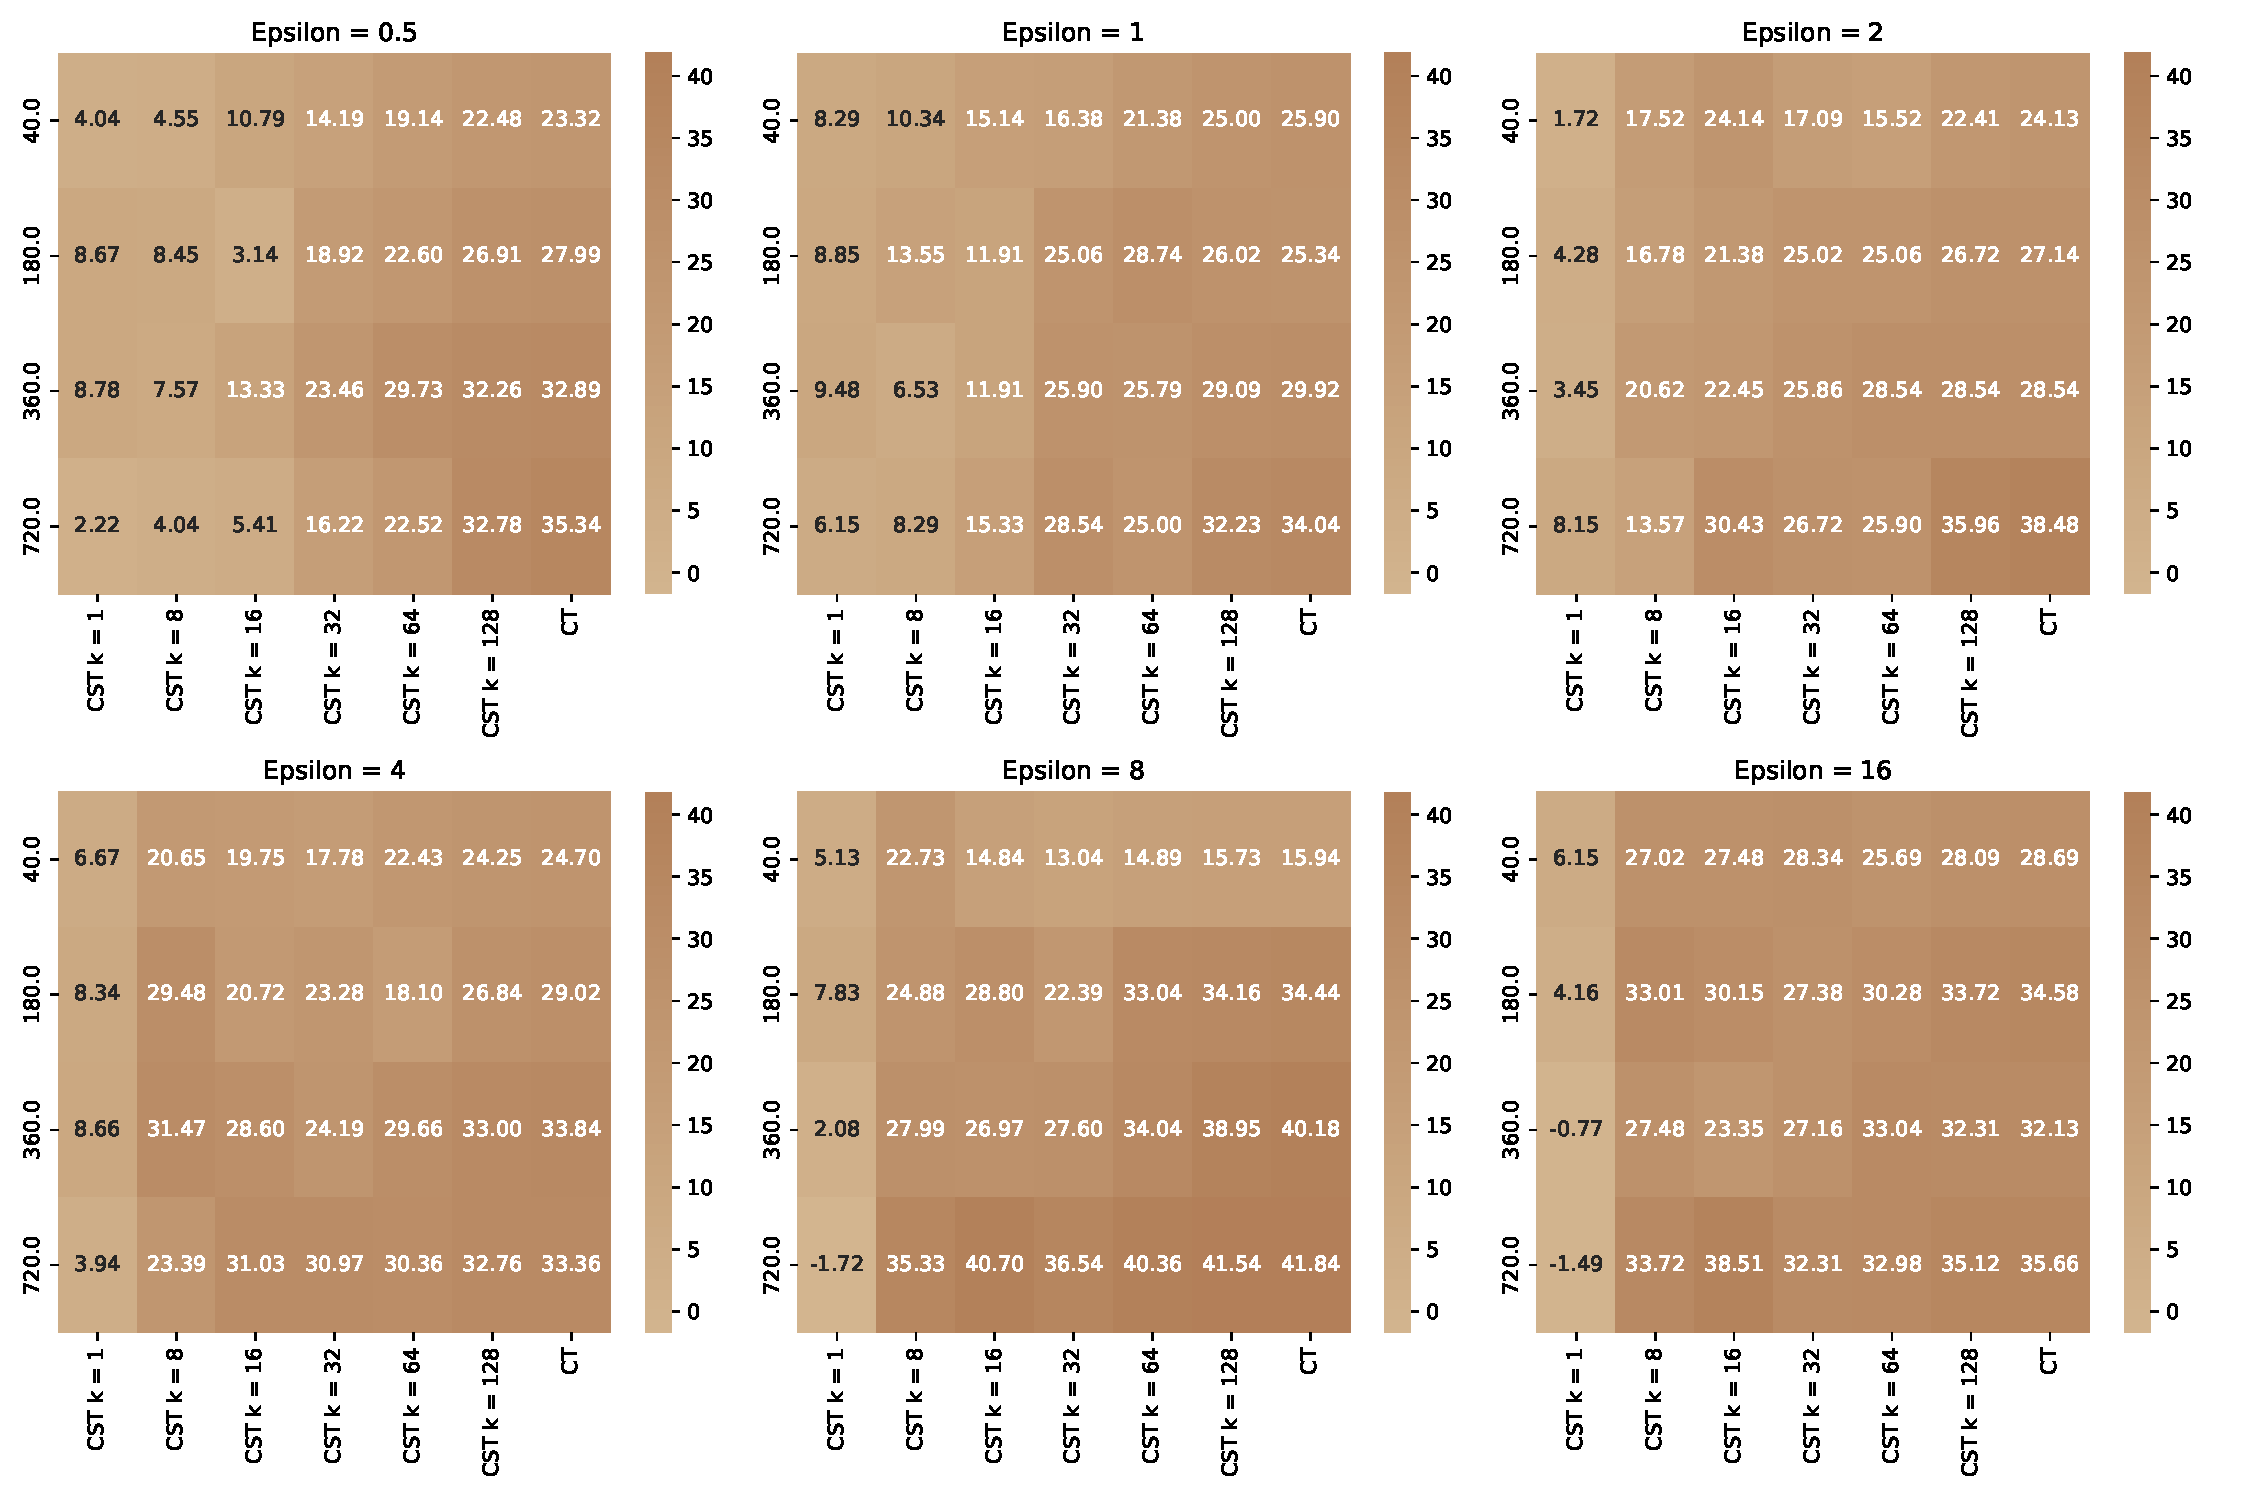
\includegraphics[width=15cm]{latex/fig/heatmap_cohesiveness.pdf}
    \caption{Cohesiveness improvement over SanText (\%); the higher, the better.}
    \label{fig:cohesiveness}
\end{figure*}

\end{document}
